\documentclass[12pt]{My_preprint}

\usetikzlibrary{arrows.meta,
                chains,
                positioning,
                shapes.geometric}
%%%%%%%%%%%%%%%%%%%%%%%%%%%%%%%%%%%%%%%%%%%%%%%%%%%%%%%%%%%%%%%%%%%%%%%%%%%%%%%
\newcommand{\size}{0.22\textwidth}
\newcommand{\avg}[1]{\left<#1\right>}
\renewcommand{\avg}[1]{\left<#1\right>}
\newcommand{\condavg}[1]{\left<#1 | \mathscr{C}_1\right>}
\newcommand{\Exp}[1]{\overline{\overline{#1}}}
\newcommand{\davg}[1]{\left<#1\right>_d}
\newcommand{\Iavg}[1]{\left<#1\right>_I}
\newcommand{\pavg}[1]{\avg{\delta_\alpha #1}}
% \newcommand{\pnavg}[1]{n\left<#1\right>_p}

\newcommand{\avgcond}[1]{\overline{#1}}
% \renewcommand{\avgcond}[1]{\left{#1}}
\newcommand{\kavg}[1]{\avgcond{#1}^k}
\newcommand{\cavg}[1]{\avgcond{#1}^c}
\newcommand{\Tavg}[1]{\avgcond{#1}^T}
\newcommand{\Xavg}[1]{\avgcond{#1}^X}
\newcommand{\TXavg}[1]{\Tavg{\Xavg{#1}}}
\newcommand{\pnnavg}[1]{\avgcond{#1}^{p}}
\newcommand{\pnavg}[1]{n_p\pnnavg{#1}}
\newcommand{\oneavg}[1]{\avgcond{#1}^1}
\newcommand{\twoavg}[1]{\avgcond{#1}^2}
\newcommand{\smallavg}[2]{\avgcond{#1}^{#2}}
\newcommand{\sym}[1]{\left(#1\right)^{\text{Sym}}}
\newcommand{\CC}{\mathscr{C}}
\newcommand{\PP}{\mathscr{P}}
\newcommand{\nstavg}[1]{\overline{#1}^\text{nst}}
\newcommand{\nstrelavg}[1]{\nstavg{#1}_\text{rel}}
\newcommand{\mavg}[1]{\left<#1\right>_m}
\newcommand{\gavg}[2][\gamma]{\left<#2\right>_{#1}}
\newcommand{\partials}[1]{\partial_{i_1}\partial_{i_2}\ldots\partial{i_{#1}}}
\newcommand{\partialp}[2]{ \prod_{m=#1}^{#2} \partial_{i_m}}
\newcommand{\hatpartialp}[2]{ \prod_{m=#1}^{#2} \hat{\partial}_{j_m}}
\newcommand{\hatpartialpi}[2]{ \prod_{m=#1}^{#2} \hat{\partial}_{i_m}}
\newcommand{\pri}[2]{ \prod_{m=#1}^{#2} r_{i_m}}
\newcommand{\prj}[2]{ \prod_{m=#1}^{#2} r_{j_m}}
\newcommand{\nablab}{\mathbf{\nabla}}
\newcommand{\nablabh}{\nablab}
\newcommand{\nablabhI}{\nablab_{||}}
\newcommand{\ddt}{\frac{d}{d t}}
\newcommand{\pddt}{\frac{\partial}{\partial t}}
\renewcommand{\pddt}{\partial_t}
\newcommand{\norm}[1]{\hat{#1}}
\newcommand{\Jump}[1]{\llbracket #1 \rrbracket \cdot \textbf{n} }

%%% Utiliser pour les commentaires
\newcommand{\JL}[1]{\color{red}#1\color{black}}
\newcommand{\SP}[1]{\color{green}#1\color{black}}
\newcommand{\tb}[1]{\color{blue}#1\color{black}}
\newcommand{\NF}[1]{\tb{#1}}

\renewcommand{\size}[1]{0.3\textwidth}
\newcommand{\expo}[2][n]{\frac{(-1)^#1}{#1!} \partialp{1}{#1} \pavg{\int_{\Omega_\alpha} \pri{1}{#1}#2 d\Omega}}
\newcommand{\expoU}[2][n]{\frac{(-1)^#1}{#1!} \partialp{1}{#1} \pavg{\textbf{u}_\alpha\int_{\Omega_\alpha} \pri{1}{#1}#2 d\Omega}}
\newcommand{\expoS}[2][n]{\frac{(-1)^#1}{#1!} \partialp{1}{#1} \pavg{\int_{\Sigma_\alpha} \pri{1}{#1}#2 d\Sigma}}


% \newcommand{\numref}[1]{\ref{#1}}
\renewcommand{\ref}[1]{\autoref{#1}}

%%%%%%%%%%%%%%%%%%%%%%%%%%%%%%% Title & Author %%%%%%%%%%%%%%%%%%%%%%%%%%%%%%%%


%\title{Reynolds stress and inertial interphase force in buoyant emulsion.}
\title{Buoyancy-driven motion of inertial monodisperse suspension of drops}
%\title{Velocity and nearest particle statistics %Buoyancy-driven motion of inertial monodisperse suspension of drops}


\author[1,2]{Nicolas Fintzi}
\author[2]{Stephane Popinet}
\author[1]{Jean-Lou Pierson}
\affil[1]{IFP Energies Nouvelles, Rond-point de l’changeur de Solaize, 69360 Solaize}
\affil[2]{Sorbonne Université, Institut Jean le Rond d’Alembert, 4 place Jussieu, 75252 PARIS CEDEX 05, France}
\normalmarginpar
\begin{document}

\maketitle

\begin{abstract}
    % We performed direct numerical simulation (DNS) of mono disperse rising droplets. 
    This article present a numerical analysis of the pseudo turbulence Reynolds stress and interphase drag force in inertial emulsion. 
    In the view of feeding averaged navier stokes model it is crucial to obtain those terms. 
    In this work new kind of algorithm which prevent coalescence between VOF tracer has been developed.
    This enables us to perform statistically steady state simulations of mono-disperse buoyant droplets for various \textit{Galileo} number $Ga = 5 \rightarrow 10$, volume fraction $\phi =1\% \rightarrow 10\%$ and viscosity ratio $\lambda = 0.1,1$. 
    By the mean of the recent concept of the nearest particle statistics \citep{zhang2021stress} we analyze meticulously the averaged flow flied around a particle and the averaged particles relative position.s 
    From this analysis we propose physical interpretation to explain the form of the closure terms.
    In this study we focus on the interphase drag and velocity fluctuation. 
\end{abstract}
\tableofcontents
\listoftodos
\begin{itemize}
    \item \tb{Kinetic energy spectra ?}
\end{itemize}



\section{Introduction}
\textbf{Objetcives : }

\begin{enumerate}
    \item Compute closure terms for buoyant emulsion
    \item Needs Statistically steady numerical experience to be representative 
    \item Therefore we introduce the no-calesence algorithm to obtain be statistically steady
    \item Allowing us to carry out massive DNS to compute closures terms. 
\end{enumerate}
\vspace*{1cm}
\textbf{notes}
\begin{itemize}
    \item biblio Lhuillier
    \item In the perspective of macroscopic modeling we have to close some terms 
    \begin{itemize}
        \item oil water processes
        \item vapour water process mu r = 6 
    \end{itemize}
    \item In the literature there is absolutely nothing for emulsion 
    \item Thus we study $Bo = 1$ $\mu_r = 0.1$ and $\rho_r = 1.11$. 
    \item Within the framework of hybrid model averaged equations in a mono-disperse case 
    \item Present theritical : 
     \begin{itemize}
        \item Momentum averaged equation for fluid particle two-fluid formulation. 
        \item Closure terms. (Merabahdi good intro)
    \end{itemize}
\end{itemize}
\todo[inline]{Introduce the dimensionless parameter in introduction to point out the gap for unity density and viscosity ratio. 
Do the same as \citet{hidman2023assessing}}

The configuration is also influenced by particle inertia. Citer Yin et Koch ... plus les papiers sur les ecoulements à bulles (Bunner et Tryggvason, Loisy)

Eventuellement citer quelques papiers en regime potentiel ? Discuter plus en details de la microstrucutre a la Jacques ?

Pour une sphere solide regime de Stokes on a n (R-Z) a ecrire. Pour des bulles ? experience a bas Re pour des bulles spheriques et non contaminees ?


Dans la suite il faut liste la biblio pour les differentes femetures ci apres
\subsection{Averaged forces}

\subsection{Velocity fluctutations}

\subsection{Stresslet and particle fluid particle stress}






%has a long history even in the Stokes regime. 





%%%%%%%%%%%%%%%%%%%%%%%%%%%%%%%%%%%%%%%%%%%%%%%%
%%%%%%%%%%%%%%%%%%%%%%%%%%%%%%%%%%%%%%%%%%%%%%%%
%\section{Theoretical context}
%

\subsection{Simulations setup}
Objective of this section :
\begin{itemize}
    \item Introduce the dimensionless parameters.
    \item Present the physical parameters of some industrial processes to locate our problematic. 
    \item Introduce the dimensionless parameters range investigated in this study.
    \item Present the tri-periodic box within which we add droplets in vof 
\end{itemize}
We investigate the dynamic of homogeneous mono-disperse emulsion subject to buoyancy forces. 
Both the dispersed (resp. continuous) phase is considered as Newtonian fluid defined by viscosity $\mu_d$ (resp. $\mu_c$), and density $\rho_d$ ($\mu_c$).
Throughout this work, the indices $d$ and $c$ indicate properties belonging to the dispersed and continuous phase, respectively. 
The interface between both fluid is considered as infinitely thin and deprived of any impurities so that it can only be described with the surface tension coefficient $\sigma$. 
In this work the density, viscosity of each phase, and surface tension coefficient, will be considered constant during  the time of a numerical experiment.
In dimensionless form the physics of the flow is described by $4$ dimensionless parameters: 
The viscosity and density ratio, $\mu_r = \mu_d / \mu_c$ and $\rho_r = \rho_d / \rho_c$, respectively. 
The \textit{Galileo} number, 
\begin{equation*}
    Ga =\sqrt{\rho_c(\rho_c - \rho_d) g d^3} / \mu_c
\end{equation*}
where $a$ is the equivalent radius of the droplets.
And the \textit{Bond} number, 
\begin{equation*}
    Bo =\frac{(\rho_c - \rho_d) g d^2}{\sigma}
\end{equation*}
with $g$ the gravity constant. 
The \textit{Galileo} number measure the influence of the buoyancy forces against the viscous forces.
Whereas the \textit{Bond} number evaluate the ratio between buoyancy and capillary forces. 
In addition to these $4$ parameters we introduce the number of particles, $N_b$, and the dispersed phase volume fraction $\phi_d$ which fully describe the topology of a finite domain of the flow. 


\begin{table}[h!]
    \centering
    \caption{Dimensionless parameter range investigated in this work.}
    \begin{tabular}{ccccccc}\hline
        $Ga$&$Bo$&$\phi$&$\mu_r$&$\rho_r$&$N_b$&$t^*_{end}$\\ \hline\hline
        $5\rightarrow 100$&$1$&$1\% \rightarrow 20\%$&$0.1 \& 1$&$1.111$&$125$&$500$\\ \hline
    \end{tabular}
    \label{tab:parameters}
\end{table}
\JL{il faut choisir entre $\mu_r$ et $\lambda$... Pr ailleurs je pense qu'l y a une coquille dans ta definition de $\mu_r$.}

We wish to investigate the moderate inertial emulsion regime with quasi spherical droplets. \todo{gives real parameters values compared to experiment ? Yes. tu peux le faire facilement en prenant par exmeple des gouttes allant de 500 microns a 2 mm. Cela ajoutera un peu de poids au choix des parametres. Par ailleurs se pose la question de lancer quelques cas à plus bas nombre de Bond (car experimentalement ils le seront) voir si cela change les resultats. De meme, pq ne pas lancer quelques cas ou les gouttes sont moins visqueuses que le fluide environnant ?}
Thus, the \textit{Bond} number must be low enough to obtain nearly spherical drops, and the viscosity and density ratio must approach the oil/water situation. 
It will be shown in the next few sections that a $Bo =1$ gives reasonable results. 
Additionally, for a statistical convergence reason explained in \ref{sec:preliminary} we choose $N_b = 125$. 
Therefore, in the following we will keep the dimensionless parameters within the ranges depicted in \ref{tab:parameters}.
In summary, we investigated $6$ \textit{Galileo} number $Ga = 5,10,25,50,75,100$, four volume fractions $\phi = 0.01,0.05,0.1,0.15,0.2$, and two viscosity ratios $\mu_r =0.1,1$. 
This makes a total of $60$ representative simulations of $125$ droplets which is expensive. 
Therefore, in the next sections we develop on our numerical strategy to make efficient multi VOF simulations. 

\tb{It is clear that at $\phi>0.1$ the mono disperse simulation aren't physicaly realistic since coalesence should arise at those volume fraction.}

To mimic infinitely large homogeneous emulsions we consider a tri periodic cubic domain of length $L$, within which, both phases are subject to the incompressible Navier Stokes equations with the corresponding boundaries conditions. To prevent an uniform acceleration of the fluids phase one need to impose a pressure gradient (or equivalently a body force) to the momentum equation. This body force may be straightforwadly obtained from the dispersed phase momentum equations. In particular in the present configurations the momentum balance simplifies to
\begin{align}
0 &= -\epsilon\frac{\partial p}{\partial z} - \rho_c \epsilon g - n_p \textbf{f}_p \label{eq:uf_triperio}
    \\
0 &= -\phi\frac{\partial p}{\partial z}     - \rho_d \phi g + n_p \textbf{f}_p \label{eq:up_triperio}
\end{align}

Adding those two equations together we obtain
\begin{equation}
-\frac{\partial p}{\partial z} = \rho_c (1-\phi) g + \rho_d \phi g 
\end{equation}











%\section{Numerical methodology}
%Introduce basilisk 
\subsection{Simulation set-up}
\begin{itemize}
    \item Introduce tri-periodic simulations
\end{itemize}
%\subsection{The no-coalescence algorithm}
Objectives 
\begin{itemize}
    \item Presents the bibliography. 
    \item Introduce mani's algorithm
    \item explain step by step the algorithm
\end{itemize}


The key feature of numerical simulations is the use of a whole new algorithm which prevent numerical coalesce of droplets to occur.
First, the reader can find the described source code at \href{https://basilisk.fr/sandbox/fintzin/no-coalesce.h}{no-coalesce.h}. 
In the following we describe the global ideas and principles, then we dive into a step by step explanation of the algorithm. 
But first some worlds on the already existing algorithm is in order.

In previous studies several methods have been used to avoid coalescence. 
The first one is to increase artificially the surface tension coefficient locally such as it is done in \citet{hidman2023assessing}.
When using a level set method to track the  phase indicator function some authors developed a multiple marker level-set method to prevent coalesence, see \citet{balcazar2015multiple}. 
Similarly, for VOF tracer some author used a multi-vof approach. 
In a recent study \citet{zhang2021direct} used one VOF tracer per bubble in his simulation which prevent coalesence and allows to track bubbles independently. 
However, this approach is quite expensive as it requires solving \ref{eq:dt_alpha} for each drop. 
Instead, we adopt the methodology of \citet{karnakov2022computing} which consider a constant number of VOF tracer with respect to the number of dorplets. 
We then adoped another methodology to track bubbles independently that we adapted inside the \texttt{Basilisk} code. 

The adaptation of  \citet{karnakov2022computing} within the basilisk code has been carried out by \citet{mani2021numerical}, which developed an algorithm to prevents the adjacent droplets to have similar VOF tracers using the least VOF tracer as possible by allowing different drops to be included within the same VOF tracer.
Specifically we define $N(t)$ VOF tracer labeled as $\alpha_d^i$ for $i =0,\ldots,N$ where $N(t)$ is dependent on time since it is function of the particles positions.  
The only requirement is that the adjacent droplets at a given time $t$, have different VOF tracer to prevent coalescence. 


\begin{figure}[h!]
    \centering
    % \begin{tikzpicture}[scale=0.1,
    %     node distance = 4mm and 6mm,
    %   start chain = going below,
    %   base/.style = {draw, thick, fill=gray!10, align=center, 
    %                  inner xsep=2mm, inner ysep=2mm},
    %   rect/.style = {base},
    %   elli/.style = {ellipse, base},
    %   circ/.style = {circle, fill=graye!10, minimum size=12pt},
    %   diam/.style = {diamond, base, aspect=1.5},
    %   line/.style = {draw, rounded corners, -Stealth, semithick},
    % ]
    % % Place nodes
    % \begin{scope}[nodes = {on chain, join=by line}]
    % \node [rect, rounded corners=10pt] (step1) {start};
    % \node [rect] (step2) {(1) Apply tag function \\ on vof field $\alpha_d^i$};
    % \node [base] (step3) {(2) Check for any adjacent drops \\ that have the same $\alpha_d^i$};
    % \node [rect] (step5) {(3) Change drops vof tracers for all\\ adjacent drops.};
    % \node [diam] (step7) {$i < N(t)$};
    % \node [rect, rounded corners=10pt] (step8) {stop};
    % \end{scope}
    % % \node [rect, left=of step3] (step9) {$i = i+1$};
    % % Draw edges
    % % \path[line] (step7) -| (step9);
    % % \path[line] (step9) |- (step2);
    % %
    % \path       (step7) -- node [right,near start]{False}    (step8);
    % \node [right=of step5] {
        % };
        % \end{tikzpicture}
    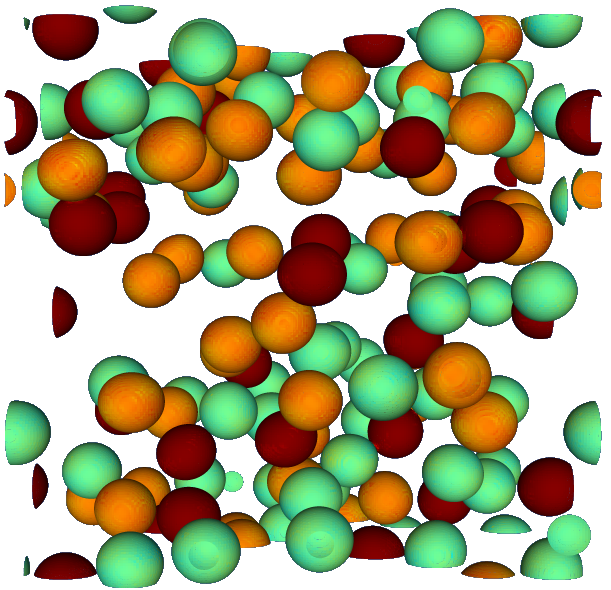
\includegraphics[width = 0.6\textwidth]{image/VOF2.png}
    \caption{
    %     Simplified flowchar of the \texttt{no-coalescence.h} algorithm.
    % $\{\alpha_d^i;i\in\mathbb{N}^{*+}\}$ represent the list of VOF tracer currently used. 
    % $N(t)$ is the total number of tracer at time $t$. 
    (b) Interface of the droplets colored by the value of $\alpha_d^i$ at $t_g =100$.
    }
    \label{fig:diagram}
\end{figure}


The simplified workflow of the algorithm follows these three steps : 
\begin{enumerate}
    \item We first identify the different topologies, i.e. the droplets, within a single tracer $\alpha_d^i$. 
    This is done by using another Basilisk feature which assign to a scalar field a different value to each topological object such as a drop (see \href{http://basilisk.fr/src/tag.h}{tag.h})\todo{biblio ?}
    \item Then we identify the droplets/tag which are different and too close to one another.
    The distance criterion is fixed to a cube of 5 mesh cells length.  
    \item Lastly we assign a new VOF tracer for each required droplets among the VOF tracer that are not already adjacent to the droplets. 
    If no VOF tracer is available we create a new one for the droplets.
    \todo{Maybe more details ?}
\end{enumerate}
This algorithm is executed at each simulation time step. 
Besides having $N$ VOF tracer require some modifications to the previously mentioned governing equations. 
Especially, instead of solving \ref{eq:dt_alpha}  we solve $N$ transport equation for each $\alpha_d^i$\todo{Is it true ?}.
But also, we compute the surface tension force as the sum of the contribution from each VOF tracer, namely, 
\begin{equation}
    \textbf{f}_\sigma \delta(\textbf{x}-\textbf{x}_I)
    = \sum_{i=0}^{N(t)} \sigma \kappa \nablab \alpha_d^i
\end{equation} 
where $\kappa_i$ is the approximate curvature of $\alpha_d^i$. 
In the 2D simulations (not presented here) we do not used more than 4 VOF tracers for hundreds of droplets during a simulation. 
This is a consequence  of the four color map theorem derived from topological arguments.
In the three-dimensional were we simulated hundreds of droplets we observed the creation of $6$ VOF tracer in the long run of the simulations.
A picture of the colored VOF is shown \ref{fig:diagram} (b) where only 3 VOF tracer is needed.
Indeed, the four color map theorem isn't valid anymore therefore the increase of VOF tracer isn't surprising anymore. 

Overall, we used an optimized multi-VOF method which allows us to compute massive DNS with approximately $6$ VOF tracers. 

\subsection{Ensemble average approximation}

Objectives : 
\begin{itemize}
    \item Present How we compute the particle properties. 
    \item Explain How we approximate the ensemble average in the numerical calculations
    \item Focus on the drag force term and on the velocity fluctuation. 
\end{itemize}

Following \citet{du2022analysis} we consider ergodicity at all time of the numerical experiment.
Thus, the ensemble average of a quantity $X$ can be approximated by a spatial average $\Xavg{X}$ and a time average $\Tavg{X}$ such that $\avg{X} = \Xavg{\Tavg{X}}=\Tavg{\Xavg{X}}$.
Consequently, the ensemble average of a numerical field, $X$, is taken through space and time such that,
\begin{equation}
    \avg{X}
    = \Tavg{\Xavg{X}}
    = \frac{1}{ t_{end} - t_0}\int_{t_0}^{t_{end}} 
    \Xavg{X}(t) dt
\end{equation}
where, 
\begin{equation}
    \Xavg{X}(t)
    = \frac{1}{L^3}\int 
    X(\textbf{x},t) d\textbf{x}
\end{equation}
where $L$ is the length of the cubic domain.
$t_0$ and $t_{end}$ is the starting time of sampling and the time duration of the simulation, respectively.
In practice, we take $t_0$ such that the simulation reach a statistically steady regime for $t>t_0$.  
Both $t_{end} $ and $t_0$ are given in \ref{ap:A} after several validations studies. 

To compute the continuous phase averaged quantities such as \ref{eq:def_uuc} we proceed as such,
\begin{equation}
    \phi_c \bm{\sigma}^{\text{Re}}_c /\rho_c
    % = \Tavg{\Xavg{\chi_c \textbf{u}_c' \textbf{u}_c'}}
    = \Tavg{\Xavg{\chi_c (\textbf{u}_c^0 -\textbf{u}_c ) (\textbf{u}_c^0 -\textbf{u}_c)}}
    = \Tavg{\Xavg{\chi_c \textbf{u}_c^0 \textbf{u}_c^0}}
    -  \phi_c  \textbf{u}_c \textbf{u}_c.
    \label{eq:def_uuc_num} 
\end{equation}
where the indicator funciton $\chi_c$ must be understood as its approximation in the DNS, i.e the color function $1 - \alpha_d$. 
Consequently, \ref{eq:def_uuc_num} indicate that we must take the average of the product of the velocities, and then we retrieve the mean velocities' product. 
Additionally,  note that the Reynolds stress can be decomposed by such as : 
\begin{align*}
    \phi_c \bm{\sigma}^{\text{Re}}_c /\rho_c
    &= 
    \Tavg{\Xavg{\chi_c (\textbf{u}_c^0 -\Xavg{\chi_c\textbf{u}_c^0} / \Xavg{\chi_c} ) (\textbf{u}_c^0 -\Xavg{\chi_c\textbf{u}_c^0} / \Xavg{\chi_c} )}}\\
    &+ \Tavg{\Xavg{\chi_c} (\Xavg{\chi_c\textbf{u}_c^0} / \Xavg{\chi_c} - \textbf{u}_c ) (\Xavg{\chi_c\textbf{u}_c^0} / \Xavg{\chi_c} - \textbf{u}_c)}\\
\end{align*}
where the first term is the space fluctuation relative to the instantaneous mean velocity of the fluid $\Xavg{\chi_c\textbf{u}_c^0} / \Xavg{\chi_c}$, and the second is the time fluctuation of the instantaneous mean velocity of the fluid. 

Similar expression can be derived for the particular phase by integrating the property over the volume of the particle which is done throught the use of the \texttt{tag.h} function, then we average on each particle at all time.





\section{Computational methodology}
%\section{Numerical procedure and problem statement}
Introduce basilisk 
\subsection{Simulation set-up}
\begin{itemize}
    \item Introduce tri-periodic simulations
\end{itemize}
\subsection{The no-coalescence algorithm}
Objectives 
\begin{itemize}
    \item Presents the bibliography. 
    \item Introduce mani's algorithm
    \item explain step by step the algorithm
\end{itemize}


The key feature of numerical simulations is the use of a whole new algorithm which prevent numerical coalesce of droplets to occur.
First, the reader can find the described source code at \href{https://basilisk.fr/sandbox/fintzin/no-coalesce.h}{no-coalesce.h}. 
In the following we describe the global ideas and principles, then we dive into a step by step explanation of the algorithm. 
But first some worlds on the already existing algorithm is in order.

In previous studies several methods have been used to avoid coalescence. 
The first one is to increase artificially the surface tension coefficient locally such as it is done in \citet{hidman2023assessing}.
When using a level set method to track the  phase indicator function some authors developed a multiple marker level-set method to prevent coalesence, see \citet{balcazar2015multiple}. 
Similarly, for VOF tracer some author used a multi-vof approach. 
In a recent study \citet{zhang2021direct} used one VOF tracer per bubble in his simulation which prevent coalesence and allows to track bubbles independently. 
However, this approach is quite expensive as it requires solving \ref{eq:dt_alpha} for each drop. 
Instead, we adopt the methodology of \citet{karnakov2022computing} which consider a constant number of VOF tracer with respect to the number of dorplets. 
We then adoped another methodology to track bubbles independently that we adapted inside the \texttt{Basilisk} code. 

The adaptation of  \citet{karnakov2022computing} within the basilisk code has been carried out by \citet{mani2021numerical}, which developed an algorithm to prevents the adjacent droplets to have similar VOF tracers using the least VOF tracer as possible by allowing different drops to be included within the same VOF tracer.
Specifically we define $N(t)$ VOF tracer labeled as $\alpha_d^i$ for $i =0,\ldots,N$ where $N(t)$ is dependent on time since it is function of the particles positions.  
The only requirement is that the adjacent droplets at a given time $t$, have different VOF tracer to prevent coalescence. 


\begin{figure}[h!]
    \centering
    % \begin{tikzpicture}[scale=0.1,
    %     node distance = 4mm and 6mm,
    %   start chain = going below,
    %   base/.style = {draw, thick, fill=gray!10, align=center, 
    %                  inner xsep=2mm, inner ysep=2mm},
    %   rect/.style = {base},
    %   elli/.style = {ellipse, base},
    %   circ/.style = {circle, fill=graye!10, minimum size=12pt},
    %   diam/.style = {diamond, base, aspect=1.5},
    %   line/.style = {draw, rounded corners, -Stealth, semithick},
    % ]
    % % Place nodes
    % \begin{scope}[nodes = {on chain, join=by line}]
    % \node [rect, rounded corners=10pt] (step1) {start};
    % \node [rect] (step2) {(1) Apply tag function \\ on vof field $\alpha_d^i$};
    % \node [base] (step3) {(2) Check for any adjacent drops \\ that have the same $\alpha_d^i$};
    % \node [rect] (step5) {(3) Change drops vof tracers for all\\ adjacent drops.};
    % \node [diam] (step7) {$i < N(t)$};
    % \node [rect, rounded corners=10pt] (step8) {stop};
    % \end{scope}
    % % \node [rect, left=of step3] (step9) {$i = i+1$};
    % % Draw edges
    % % \path[line] (step7) -| (step9);
    % % \path[line] (step9) |- (step2);
    % %
    % \path       (step7) -- node [right,near start]{False}    (step8);
    % \node [right=of step5] {
        % };
        % \end{tikzpicture}
    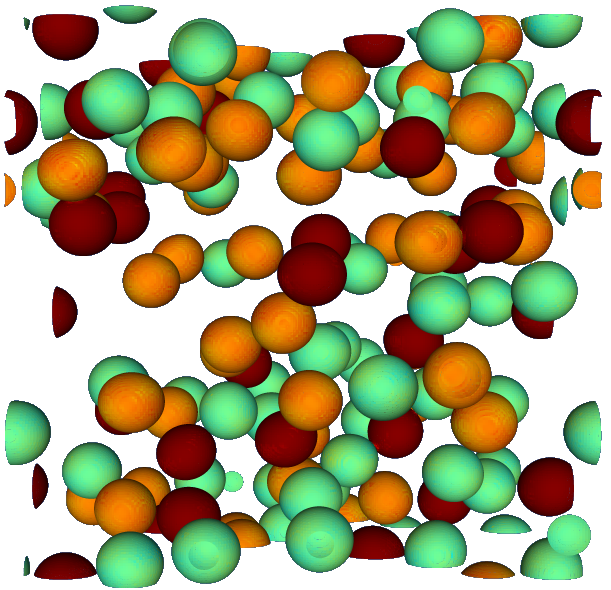
\includegraphics[width = 0.6\textwidth]{image/VOF2.png}
    \caption{
    %     Simplified flowchar of the \texttt{no-coalescence.h} algorithm.
    % $\{\alpha_d^i;i\in\mathbb{N}^{*+}\}$ represent the list of VOF tracer currently used. 
    % $N(t)$ is the total number of tracer at time $t$. 
    (b) Interface of the droplets colored by the value of $\alpha_d^i$ at $t_g =100$.
    }
    \label{fig:diagram}
\end{figure}


The simplified workflow of the algorithm follows these three steps : 
\begin{enumerate}
    \item We first identify the different topologies, i.e. the droplets, within a single tracer $\alpha_d^i$. 
    This is done by using another Basilisk feature which assign to a scalar field a different value to each topological object such as a drop (see \href{http://basilisk.fr/src/tag.h}{tag.h})\todo{biblio ?}
    \item Then we identify the droplets/tag which are different and too close to one another.
    The distance criterion is fixed to a cube of 5 mesh cells length.  
    \item Lastly we assign a new VOF tracer for each required droplets among the VOF tracer that are not already adjacent to the droplets. 
    If no VOF tracer is available we create a new one for the droplets.
    \todo{Maybe more details ?}
\end{enumerate}
This algorithm is executed at each simulation time step. 
Besides having $N$ VOF tracer require some modifications to the previously mentioned governing equations. 
Especially, instead of solving \ref{eq:dt_alpha}  we solve $N$ transport equation for each $\alpha_d^i$\todo{Is it true ?}.
But also, we compute the surface tension force as the sum of the contribution from each VOF tracer, namely, 
\begin{equation}
    \textbf{f}_\sigma \delta(\textbf{x}-\textbf{x}_I)
    = \sum_{i=0}^{N(t)} \sigma \kappa \nablab \alpha_d^i
\end{equation} 
where $\kappa_i$ is the approximate curvature of $\alpha_d^i$. 
In the 2D simulations (not presented here) we do not used more than 4 VOF tracers for hundreds of droplets during a simulation. 
This is a consequence  of the four color map theorem derived from topological arguments.
In the three-dimensional were we simulated hundreds of droplets we observed the creation of $6$ VOF tracer in the long run of the simulations.
A picture of the colored VOF is shown \ref{fig:diagram} (b) where only 3 VOF tracer is needed.
Indeed, the four color map theorem isn't valid anymore therefore the increase of VOF tracer isn't surprising anymore. 

Overall, we used an optimized multi-VOF method which allows us to compute massive DNS with approximately $6$ VOF tracers. 

\subsection{Ensemble average approximation}

Objectives : 
\begin{itemize}
    \item Present How we compute the particle properties. 
    \item Explain How we approximate the ensemble average in the numerical calculations
    \item Focus on the drag force term and on the velocity fluctuation. 
\end{itemize}

Following \citet{du2022analysis} we consider ergodicity at all time of the numerical experiment.
Thus, the ensemble average of a quantity $X$ can be approximated by a spatial average $\Xavg{X}$ and a time average $\Tavg{X}$ such that $\avg{X} = \Xavg{\Tavg{X}}=\Tavg{\Xavg{X}}$.
Consequently, the ensemble average of a numerical field, $X$, is taken through space and time such that,
\begin{equation}
    \avg{X}
    = \Tavg{\Xavg{X}}
    = \frac{1}{ t_{end} - t_0}\int_{t_0}^{t_{end}} 
    \Xavg{X}(t) dt
\end{equation}
where, 
\begin{equation}
    \Xavg{X}(t)
    = \frac{1}{L^3}\int 
    X(\textbf{x},t) d\textbf{x}
\end{equation}
where $L$ is the length of the cubic domain.
$t_0$ and $t_{end}$ is the starting time of sampling and the time duration of the simulation, respectively.
In practice, we take $t_0$ such that the simulation reach a statistically steady regime for $t>t_0$.  
Both $t_{end} $ and $t_0$ are given in \ref{ap:A} after several validations studies. 

To compute the continuous phase averaged quantities such as \ref{eq:def_uuc} we proceed as such,
\begin{equation}
    \phi_c \bm{\sigma}^{\text{Re}}_c /\rho_c
    % = \Tavg{\Xavg{\chi_c \textbf{u}_c' \textbf{u}_c'}}
    = \Tavg{\Xavg{\chi_c (\textbf{u}_c^0 -\textbf{u}_c ) (\textbf{u}_c^0 -\textbf{u}_c)}}
    = \Tavg{\Xavg{\chi_c \textbf{u}_c^0 \textbf{u}_c^0}}
    -  \phi_c  \textbf{u}_c \textbf{u}_c.
    \label{eq:def_uuc_num} 
\end{equation}
where the indicator funciton $\chi_c$ must be understood as its approximation in the DNS, i.e the color function $1 - \alpha_d$. 
Consequently, \ref{eq:def_uuc_num} indicate that we must take the average of the product of the velocities, and then we retrieve the mean velocities' product. 
Additionally,  note that the Reynolds stress can be decomposed by such as : 
\begin{align*}
    \phi_c \bm{\sigma}^{\text{Re}}_c /\rho_c
    &= 
    \Tavg{\Xavg{\chi_c (\textbf{u}_c^0 -\Xavg{\chi_c\textbf{u}_c^0} / \Xavg{\chi_c} ) (\textbf{u}_c^0 -\Xavg{\chi_c\textbf{u}_c^0} / \Xavg{\chi_c} )}}\\
    &+ \Tavg{\Xavg{\chi_c} (\Xavg{\chi_c\textbf{u}_c^0} / \Xavg{\chi_c} - \textbf{u}_c ) (\Xavg{\chi_c\textbf{u}_c^0} / \Xavg{\chi_c} - \textbf{u}_c)}\\
\end{align*}
where the first term is the space fluctuation relative to the instantaneous mean velocity of the fluid $\Xavg{\chi_c\textbf{u}_c^0} / \Xavg{\chi_c}$, and the second is the time fluctuation of the instantaneous mean velocity of the fluid. 

Similar expression can be derived for the particular phase by integrating the property over the volume of the particle which is done throught the use of the \texttt{tag.h} function, then we average on each particle at all time.




%\section{Preliminary tests}
%\label{sec:preliminary}


The \texttt{Basilisk} code has been validated numerous time in previous numerical studies \todo{Add biblio}\citet{innocenti2020direct},\citet{popinet2018numerical}. 
Therefore,  in this section we start by presenting a brief comparison with previous numerical studies. 
Afterward we present a meticulous study focusing on the interfaces dynamics, by comparing our results with the experimental results of \citet{mohamed2003drop} 
To complete these valildation we present in \ref{ap:A} several classic cases analyzing :
(1) The mesh definition, (2) The statistical time convergence, (3) the number of particles on random array of droplets. 
 
\subsection{Fixed array of bubbles}
Objectives :
\begin{itemize}
    \item Mesh validation : our DNS Vs. DNS of \cite{esmaeeli1999direct}
\end{itemize}
From our knowledge, no simulations nor experimental results have been carried out for rising buoyant viscous drop. 
Therefore, instead we reproduced the well known ordered array simulation of \citet{esmaeeli1999direct} with Basilisk to validate the mesh definition.  
It consists in a 3-D buoyant ordered rising array of bubbles. 
In our notation the flow parameters of the simulation reads, 
\begin{align*}
    \mu_r = 10,
    && \rho_r = 10,
    && Bo = 1.8,
    && Ga = 28.37,
    && \phi = 0.125.
\end{align*}
\begin{figure}[h!]
    \centering
    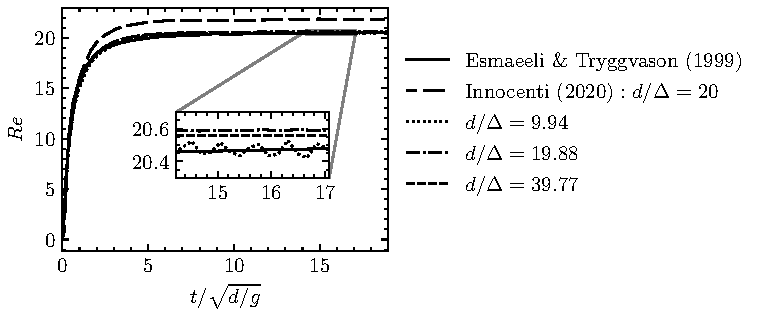
\includegraphics[height = 0.35\textwidth]{image/VALIDATION2.0/Loisy/Re.pdf}
    \caption{Time evolution of the Reynolds number based on the instentaneous volume averaged drift velocity, $Re(t) = \rho_fU d /\mu_f$, with $U(t) = (\Xavg{\textbf{u}_p} - \Xavg{\textbf{u}_c})\cdot \textbf{e}_y$ with $\phi = 0.1256$ ,$\rho_r =\mu_r =10$ and $Ga = 29.9$.}
    \label{fig:ordered_array}
\end{figure}
\ref{fig:ordered_array} display our numerical simulation against the original result of \citet{esmaeeli1999direct}
We observe very good agreements between both studies for all mesh definition.
Additionally, we displayed the results of \citet{innocenti2020direct} for $d/\Delta = 20$ to point out a divergence with our results.  
Both our simulations and the one of \citet{innocenti2020direct} have been carried out with the  \texttt{Basilisk} code. 
The cause of this difference is in fact due to a different method of interpolation used for the viscosity coefficient. 
We used an arithmetic mean, whereas \citet{innocenti2020direct} used a 
harmonic mean. 
As a matter of fact in this regime the arithmetic mean for the kinematic viscosity coefficient permit us to reach a faster convergence. 

Overall these results indicate that the criterion $d/\Delta = 30$ seems sufficient.
\todo[inline]{we could compare with bubbly flow of \citet{zhang2021direct}/\citet{roghair2011drag} \textbf{multi-vof} ? ?  }

\subsection{Drop impact on a liquid–liquid interface}
Objective : 
\begin{itemize}
    \item problematic "Do we describe well the film physics with the coalescence algorithm".
    \item Introduce the numerical set up 
    \item Comparison of the kinematic with \citet{mohamed2003drop}.  
\end{itemize}

In section we investigate in more detail the physics behind the mult-vof method. 
Indeed, we also need to check if we capture enough physics despite the fact that we do not model accurately  the film between two droplets. 
To do so we reproduced the case drop impact on a liquid–liquid interface of \citet{mohamed2003drop} as it is approximately in the range of our dimensionless numbers. 
In our notation the dimensionless parameters reads, 
\begin{align*}
    Ga = 71.02 
    && Bo = 6.40
    && \lambda = 0.33
    && \rho_r = 1.189
\end{align*}
Regarding the geometry of the problem we sceatched \ref{fig:schemeLong} the initial position of the droplet in the computational domain.
Following \citet{mohamed2003drop} we defined the dimensionless time $t / t_i = t U_i /D$ where $U_i$ is droplet velocity at $t<0$ where $t=0$ is the time of impact. 
\begin{figure}[h!]
    \centering
    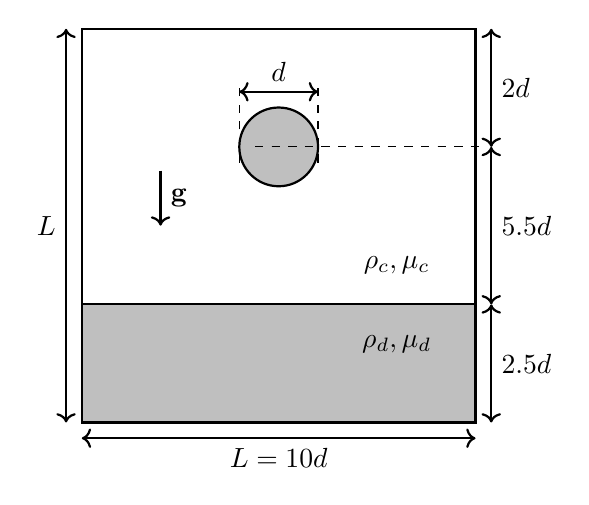
\begin{tikzpicture}[thick]
        \draw (0,0) rectangle (5,5);
        \draw[fill=gray!50] (0,0) rectangle (5,1.5);
        \draw[fill=gray!50] (2.5,3.5) circle (0.5);
        \draw[<->](0,-0.2) --++ (5,0)node[midway,below]{$L  = 10 d$};
        \draw[<->](-0.2,0) --++ (0,5)node[midway,left]{$L$};
        \draw[<->](5.2,0) --++ (0,1.5)node[midway,right]{$2.5 d$};
        \draw[<->](5.2,1.5) --++ (0,2)node[midway,right]{$5.5 d$};
        \draw[<->](5.2,3.5) --++ (0,1.5)node[midway,right]{$ 2d$};
        \draw[dashed,thin](2.2,3.5) --++ (2.9,0);
        \draw[dashed,thin](2.2,3.5) --++ (2.9,0);
        \draw[->](1,3.2) --++ (0,-0.7)node[midway,right]{$\textbf{g}$};
        \draw[<->](2,4.2) --++ (1,0)node[midway,above]{$d$};
        \draw[thin,dashed](2,3.3) --++ (0,1);
        \draw[thin,dashed](3,3.3) --++ (0,1);
        \node (a) at (4,2){$\rho_c, \mu_c$};
        \node (a) at (4,1){$\rho_d, \mu_d$};
    \end{tikzpicture}
    \caption{(left) Scheme of the computational set up at the initial time. (right) picture of the computational domain with the interfaces represented in grey.}
    \label{fig:schemeLong}
\end{figure}
\begin{figure}[h!]
    \centering
    \begin{tikzpicture}
        \node (img1) at (0,0.35\textwidth)             {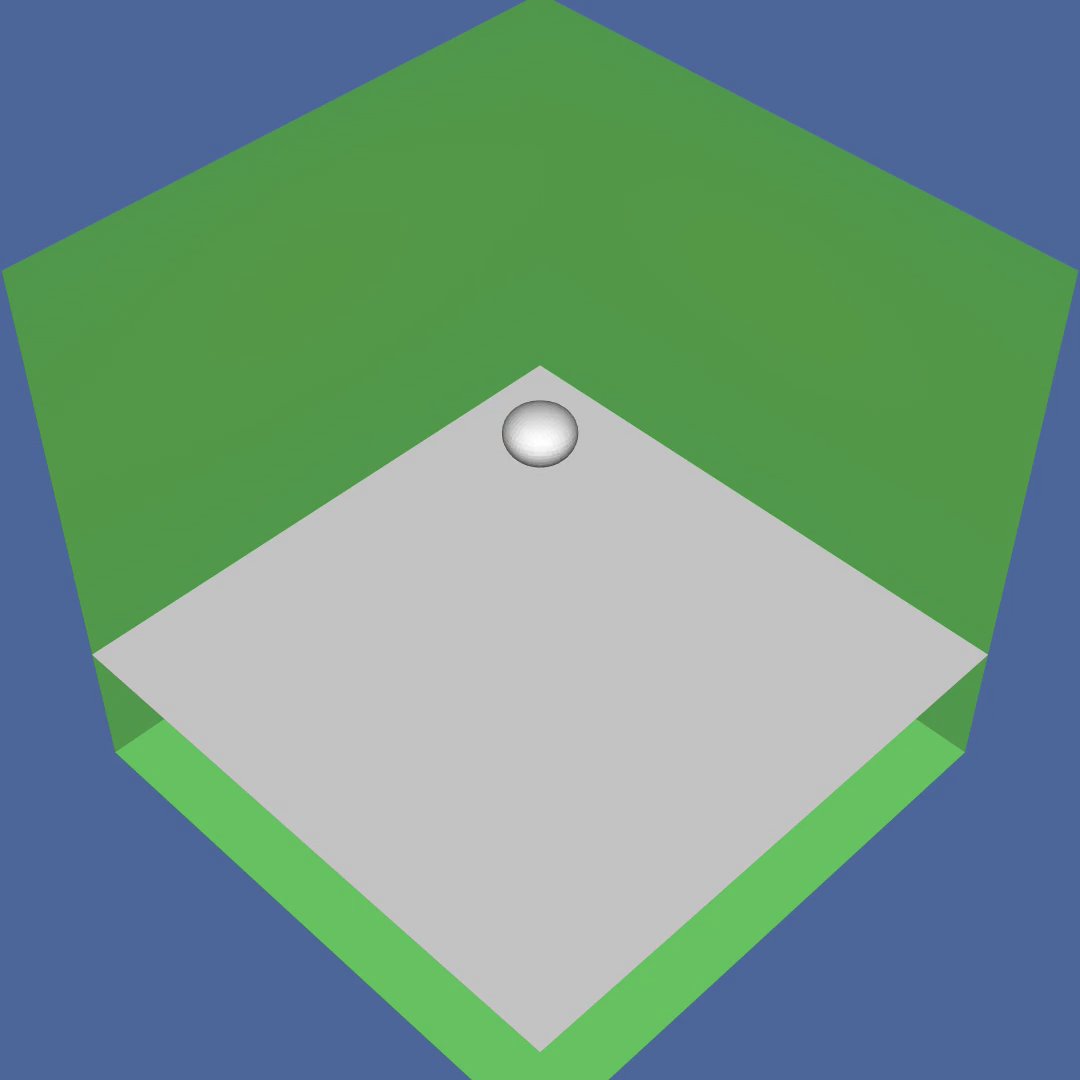
\includegraphics[height = 0.3\textwidth]{image/VALIDATION2.0/Longmire/IMG/image-010.png}};
        \node (img2) at (0.35\textwidth,0.35\textwidth) {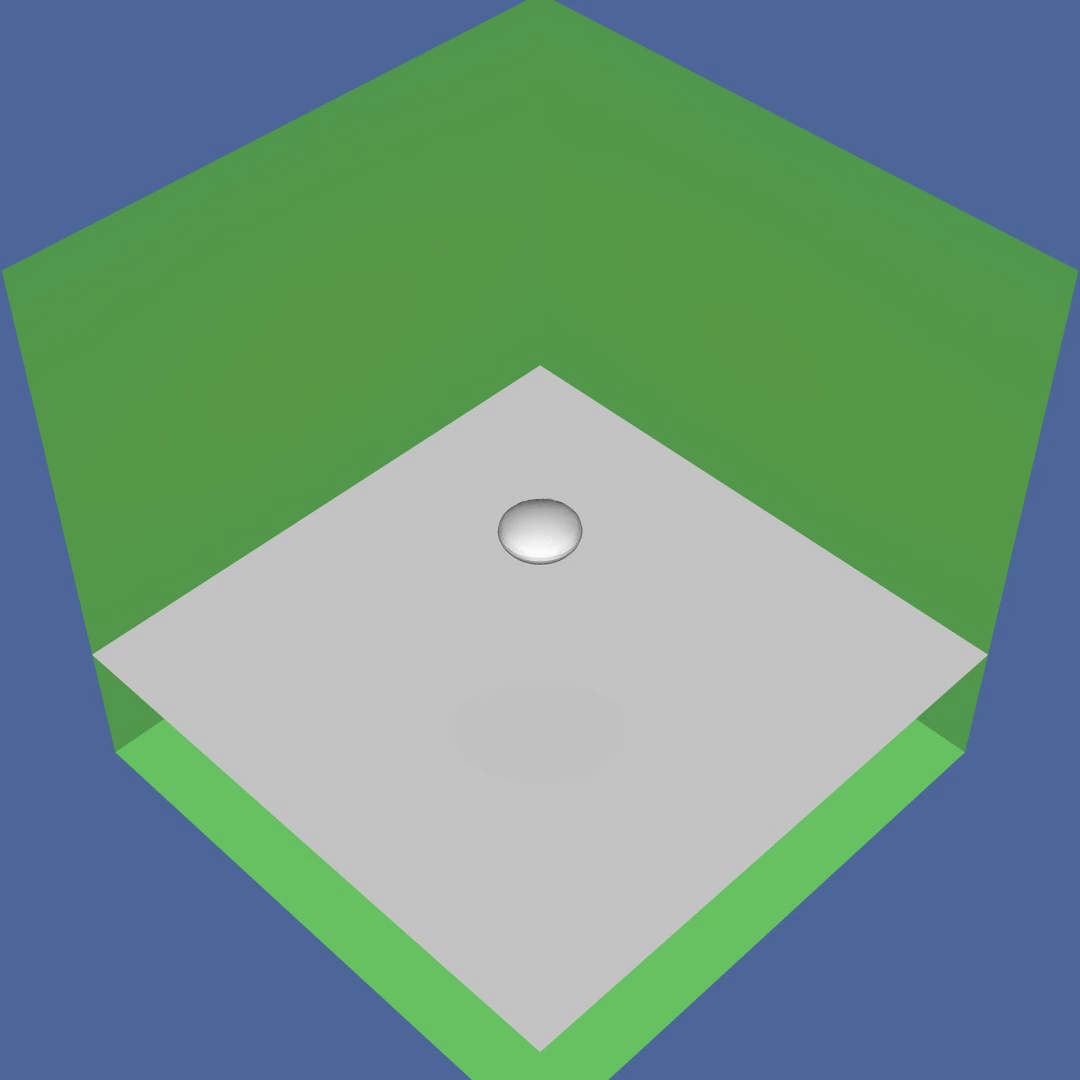
\includegraphics[height = 0.3\textwidth]{image/VALIDATION2.0/Longmire/IMG/image-020.png}};
        \node (img3) at (0.7\textwidth,0.35\textwidth) {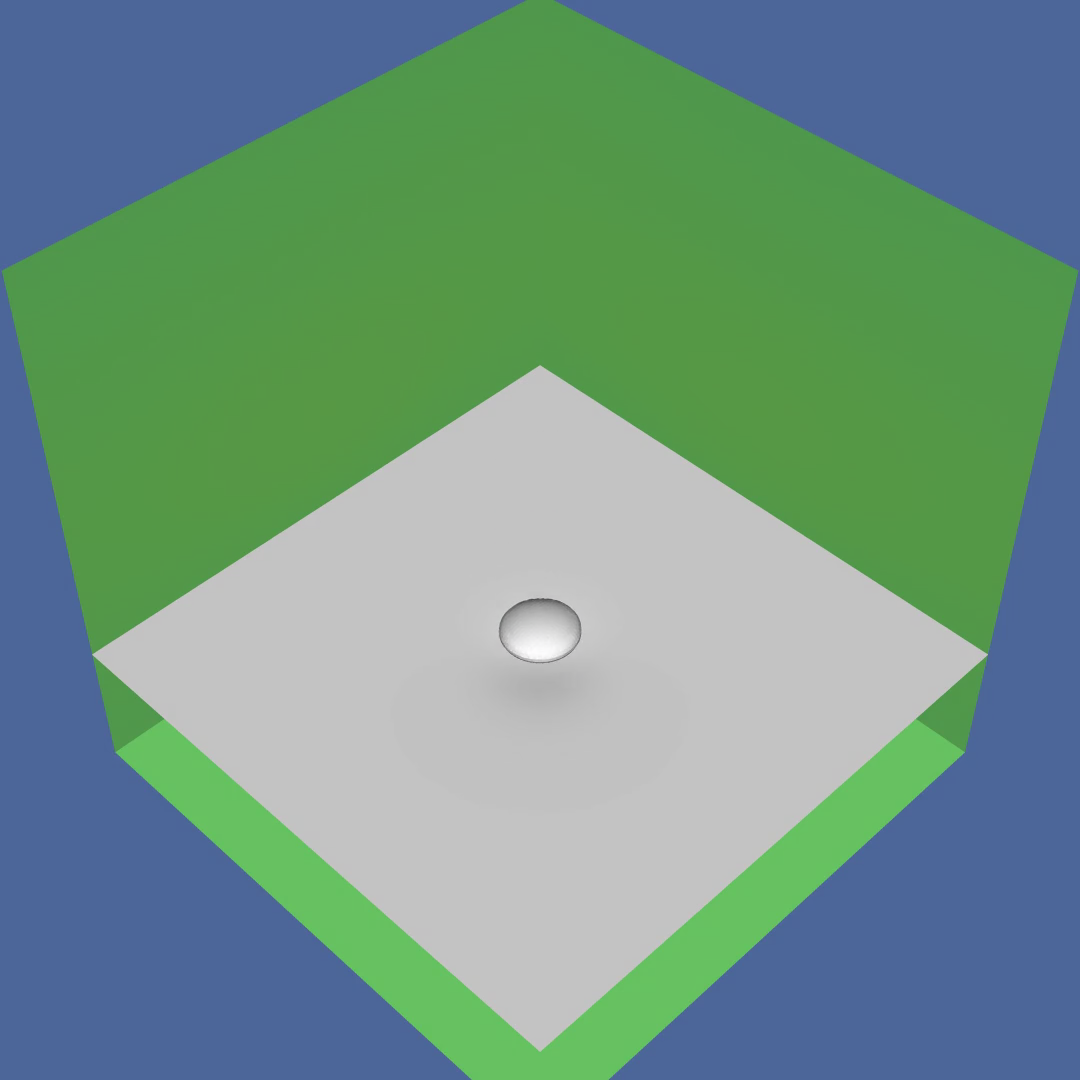
\includegraphics[height = 0.3\textwidth]{image/VALIDATION2.0/Longmire/IMG/image-030.png}};
        \node (img4) at (0,0)                         {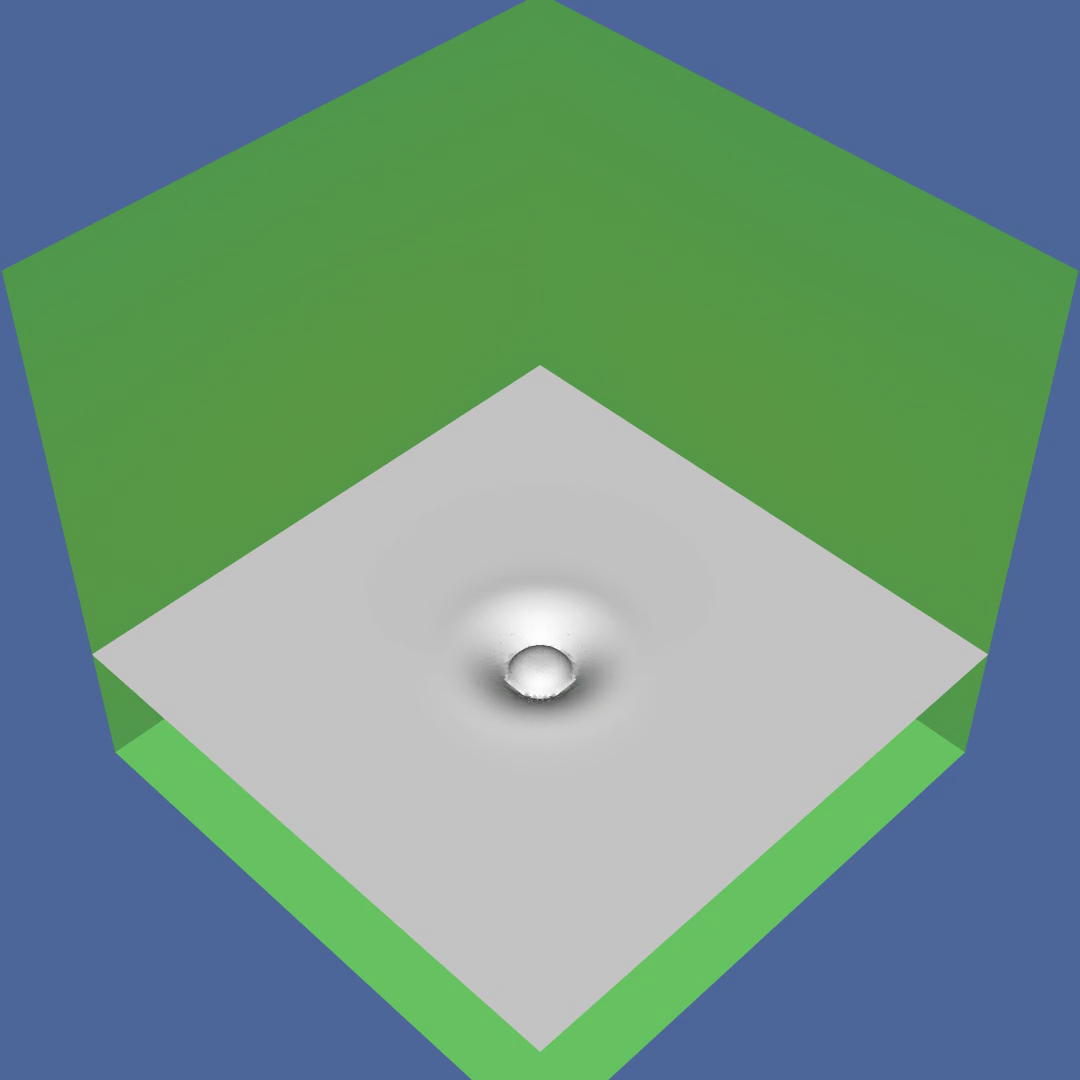
\includegraphics[height = 0.3\textwidth]{image/VALIDATION2.0/Longmire/IMG/image-040.png}};
        \node (img5) at (0.35\textwidth,0)             {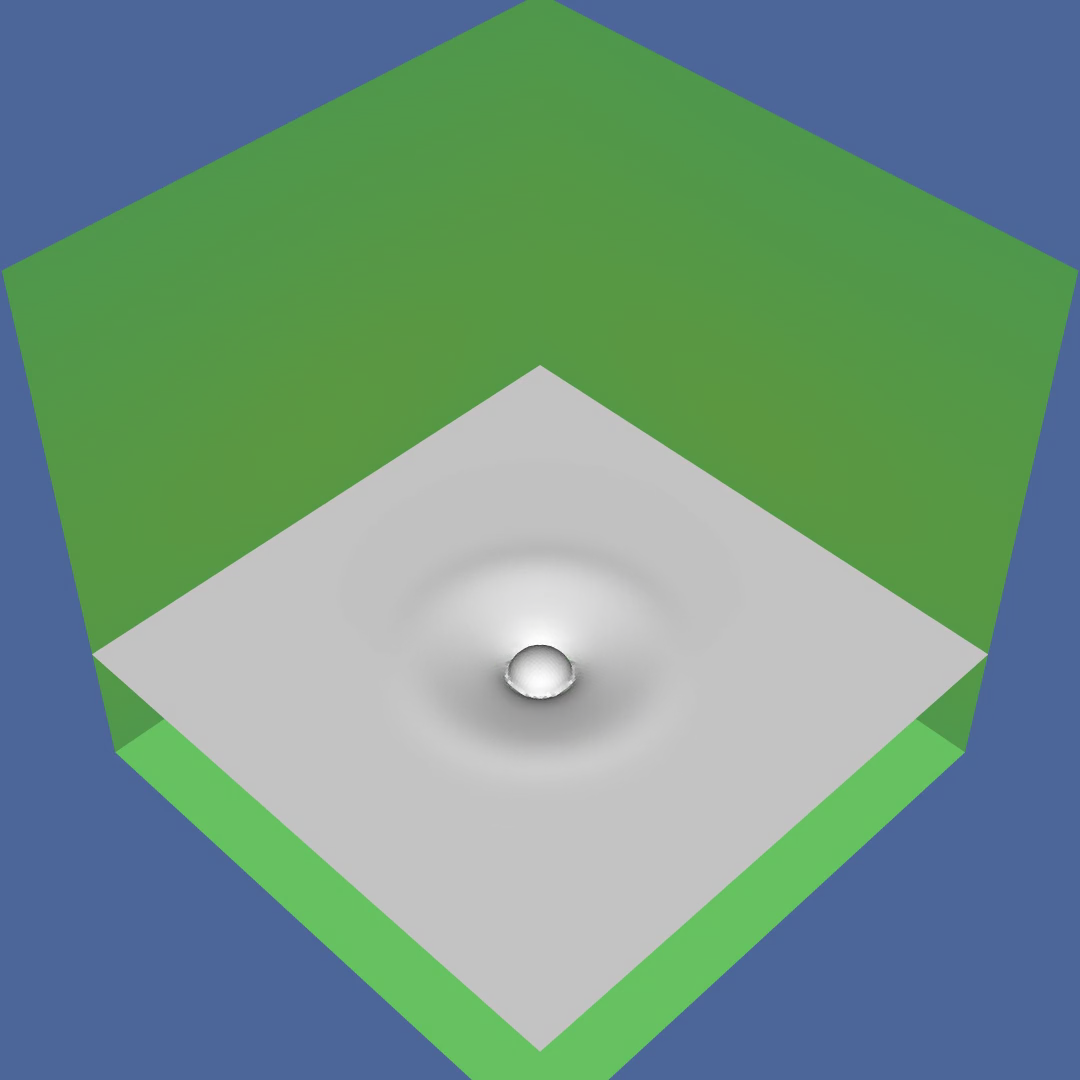
\includegraphics[height = 0.3\textwidth]{image/VALIDATION2.0/Longmire/IMG/image-050.png}};
        \node (img6) at (0.7\textwidth,0)             {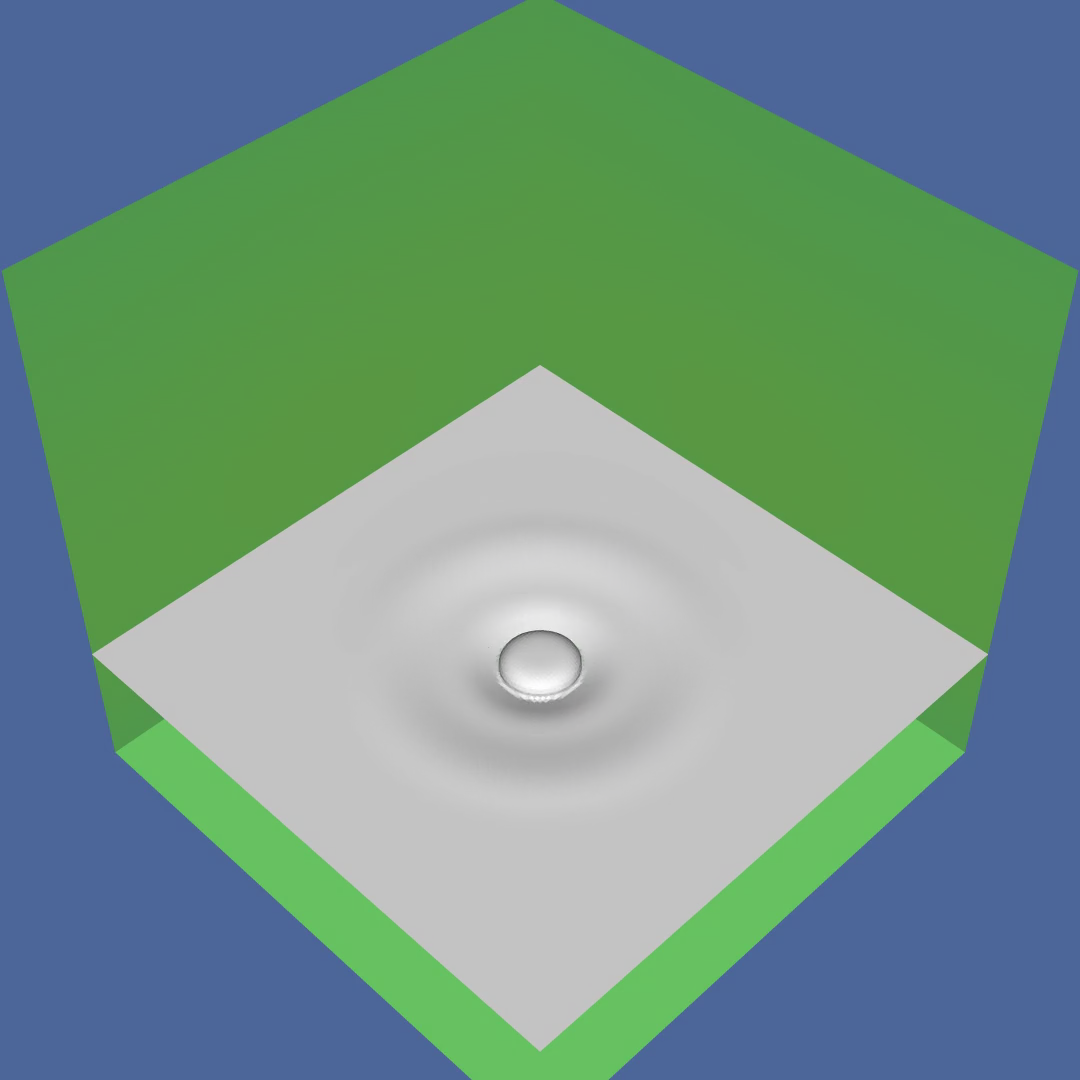
\includegraphics[height = 0.3\textwidth]{image/VALIDATION2.0/Longmire/IMG/image-060.png}};
        \node[below] at (img1.south){$t_i = -5.5$};
        \node[below] at (img2.south){$t_i = -2$};
        \node[below] at (img3.south){$t_i = 0$};
        \node[below] at (img4.south){$t_i = 2.5$};
        \node[below] at (img5.south){$t_i = 5$};
        \node[below] at (img6.south){$t_i = 15$};
    \end{tikzpicture}

    % \centering
    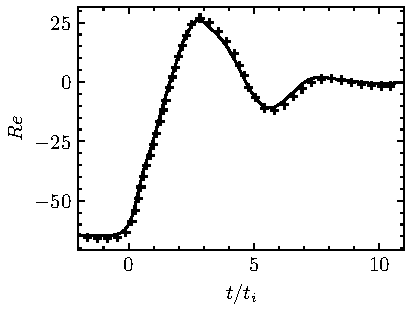
\includegraphics[height = 0.35\textwidth]{image/VALIDATION2.0/Longmire/Re.pdf}
    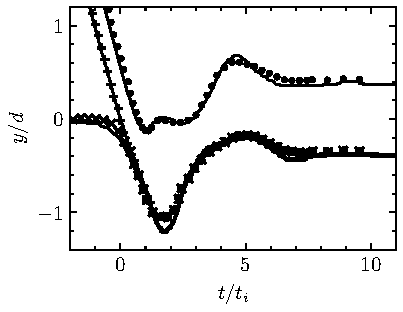
\includegraphics[height = 0.35\textwidth]{image/VALIDATION2.0/Longmire/Dist.pdf}
    \caption{(left) Time evolution of the Reynolds number based on the droplet velocity, $Re(t) = \rho_fU d /\mu_f$ in term of the dimensionless time, (+) numerical results of  \citet{balcazar2015multiple} (right)  position of the interfaces, ($\bullet$) top droplets surface, ($+$) bot droplet surface, (x) pool surface. (Symbols) experimental result of \citet{mohamed2003drop} (solid line) present numerical simulations with $d/\Delta = 30$. }
    \label{fig:resultslong}
\end{figure}
\ref{fig:resultslong} represent the comparison between our results aigainst the experiment of \citet{mohamed2003drop} (right) and the numerical simulation of \citet{balcazar2015multiple} (left). 
From the very good agreement obtained with the numerical and experimental results we conclude that the kinematic is preserved during the contact time for a mesh definition of $d/\Delta = 30$. 





\subsection{Simulations setup}
Objective of this section :
\begin{itemize}
    \item Introduce the dimensionless parameters.
    \item Present the physical parameters of some industrial processes to locate our problematic. 
    \item Introduce the dimensionless parameters range investigated in this study.
    \item Present the tri-periodic box within which we add droplets in vof 
\end{itemize}
We investigate the dynamic of homogeneous mono-disperse emulsion subject to buoyancy forces. 
Both the dispersed (resp. continuous) phase is considered as Newtonian fluid defined by viscosity $\mu_d$ (resp. $\mu_c$), and density $\rho_d$ ($\mu_c$).
Throughout this work, the indices $d$ and $c$ indicate properties belonging to the dispersed and continuous phase, respectively. 
The interface between both fluid is considered as infinitely thin and deprived of any impurities so that it can only be described with the surface tension coefficient $\sigma$. 
In this work the density, viscosity of each phase, and surface tension coefficient, will be considered constant during  the time of a numerical experiment.
In dimensionless form the physics of the flow is described by $4$ dimensionless parameters: 
The viscosity and density ratio, $\mu_r = \mu_d / \mu_c$ and $\rho_r = \rho_d / \rho_c$, respectively. 
The \textit{Galileo} number, 
\begin{equation*}
    Ga =\sqrt{\rho_c(\rho_c - \rho_d) g d^3} / \mu_c
\end{equation*}
where $a$ is the equivalent radius of the droplets.
And the \textit{Bond} number, 
\begin{equation*}
    Bo =\frac{(\rho_c - \rho_d) g d^2}{\sigma}
\end{equation*}
with $g$ the gravity constant. 
The \textit{Galileo} number measure the influence of the buoyancy forces against the viscous forces.
Whereas the \textit{Bond} number evaluate the ratio between buoyancy and capillary forces. 
In addition to these $4$ parameters we introduce the number of particles, $N_b$, and the dispersed phase volume fraction $\phi_d$ which fully describe the topology of a finite domain of the flow. 


\begin{table}[h!]
    \centering
    \caption{Dimensionless parameter range investigated in this work.}
    \begin{tabular}{ccccccc}\hline
        $Ga$&$Bo$&$\phi$&$\mu_r$&$\rho_r$&$N_b$&$t^*_{end}$\\ \hline\hline
        $5\rightarrow 100$&$1$&$1\% \rightarrow 20\%$&$0.1 \& 1$&$1.111$&$125$&$500$\\ \hline
    \end{tabular}
    \label{tab:parameters}
\end{table}
\JL{il faut choisir entre $\mu_r$ et $\lambda$... Pr ailleurs je pense qu'l y a une coquille dans ta definition de $\mu_r$.}

We wish to investigate the moderate inertial emulsion regime with quasi spherical droplets. \todo{gives real parameters values compared to experiment ? Yes. tu peux le faire facilement en prenant par exmeple des gouttes allant de 500 microns a 2 mm. Cela ajoutera un peu de poids au choix des parametres. Par ailleurs se pose la question de lancer quelques cas à plus bas nombre de Bond (car experimentalement ils le seront) voir si cela change les resultats. De meme, pq ne pas lancer quelques cas ou les gouttes sont moins visqueuses que le fluide environnant ?}
Thus, the \textit{Bond} number must be low enough to obtain nearly spherical drops, and the viscosity and density ratio must approach the oil/water situation. 
It will be shown in the next few sections that a $Bo =1$ gives reasonable results. 
Additionally, for a statistical convergence reason explained in \ref{sec:preliminary} we choose $N_b = 125$. 
Therefore, in the following we will keep the dimensionless parameters within the ranges depicted in \ref{tab:parameters}.
In summary, we investigated $6$ \textit{Galileo} number $Ga = 5,10,25,50,75,100$, four volume fractions $\phi = 0.01,0.05,0.1,0.15,0.2$, and two viscosity ratios $\mu_r =0.1,1$. 
This makes a total of $60$ representative simulations of $125$ droplets which is expensive. 
Therefore, in the next sections we develop on our numerical strategy to make efficient multi VOF simulations. 

\tb{It is clear that at $\phi>0.1$ the mono disperse simulation aren't physicaly realistic since coalesence should arise at those volume fraction.}

To mimic infinitely large homogeneous emulsions we consider a tri periodic cubic domain of length $L$, within which, both phases are subject to the incompressible Navier Stokes equations with the corresponding boundaries conditions. To prevent an uniform acceleration of the fluids phase one need to impose a pressure gradient (or equivalently a body force) to the momentum equation. This body force may be straightforwadly obtained from the dispersed phase momentum equations. In particular in the present configurations the momentum balance simplifies to
\begin{align}
0 &= -\epsilon\frac{\partial p}{\partial z} - \rho_c \epsilon g - n_p \textbf{f}_p \label{eq:uf_triperio}
    \\
0 &= -\phi\frac{\partial p}{\partial z}     - \rho_d \phi g + n_p \textbf{f}_p \label{eq:up_triperio}
\end{align}

Adding those two equations together we obtain
\begin{equation}
-\frac{\partial p}{\partial z} = \rho_c (1-\phi) g + \rho_d \phi g 
\end{equation}











\subsection{Statistics computations}

Objectives : 
\begin{itemize}
    \item Present How we compute the particle properties. 
    \item Explain How we approximate the ensemble average in the numerical calculations
    \item Focus on the drag force term and on the velocity fluctuation. 
\end{itemize}

Following \citet{du2022analysis} we consider ergodicity at all time of the numerical experiment.
Thus, the ensemble average of a quantity $X$ can be approximated by a spatial average $\Xavg{X}$ and a time average $\Tavg{X}$ such that $\int X d\PP = \avg{X} \approx \Xavg{\Tavg{X}} = \Tavg{\Xavg{X}}$.
Consequently, the ensemble average of a numerical field, $X$, is taken through space and time such that,
\begin{equation}
    \avg{X}
    = \Tavg{\Xavg{X}}
    = \frac{1}{ t_{end} - t_0}\int_{t_0}^{t_{end}} 
    \Xavg{X}(t) dt
\end{equation}
where, 
\begin{equation}
    \Xavg{X}(t)
    = \frac{1}{L^3}\int 
    X(\textbf{x},t) d\textbf{x}
\end{equation}
where $L$ is the length of the cubic domain.
$t_0$ and $t_{end}$ is the starting time of sampling and the time duration of the simulation, respectively.
In practice, we take $t_0$ such that the simulation reach a statistically steady regime for $t>t_0$.  
Both $t_{end} $ and $t_0$ are given in \ref{ap:A} after several validations studies. 

To compute the continuous phase averaged quantities such as \ref{eq:def_uuc} we proceed as such,
\begin{equation}
    \phi_c \bm{\sigma}^{\text{Re}}_c /\rho_c
    % = \Tavg{\Xavg{\chi_c \textbf{u}_c' \textbf{u}_c'}}
    = \Tavg{\Xavg{\chi_c (\textbf{u}_c^0 -\textbf{u}_c ) (\textbf{u}_c^0 -\textbf{u}_c)}}
    = \Tavg{\Xavg{\chi_c \textbf{u}_c^0 \textbf{u}_c^0}}
    -  \phi_c  \textbf{u}_c \textbf{u}_c.
    \label{eq:def_uuc_num} 
\end{equation}
where the indicator funciton $\chi_c$ must be understood as its approximation in the DNS, i.e the color function $1 - \alpha_d$. 
Consequently, \ref{eq:def_uuc_num} indicate that we must take the average of the product of the velocities, and then we retrieve the mean velocities' product. 
Additionally,  note that the Reynolds stress can be decomposed by such as : 
\begin{align*}
    \phi_c \bm{\sigma}^{\text{Re}}_c /\rho_c
    &= 
    \Tavg{\Xavg{\chi_c (\textbf{u}_c^0 -\Xavg{\chi_c\textbf{u}_c^0} / \Xavg{\chi_c} ) (\textbf{u}_c^0 -\Xavg{\chi_c\textbf{u}_c^0} / \Xavg{\chi_c} )}}\\
    &+ \Tavg{\Xavg{\chi_c} (\Xavg{\chi_c\textbf{u}_c^0} / \Xavg{\chi_c} - \textbf{u}_c ) (\Xavg{\chi_c\textbf{u}_c^0} / \Xavg{\chi_c} - \textbf{u}_c)}\\
\end{align*}
where the first term is the space fluctuation relative to the instantaneous mean velocity of the fluid $\Xavg{\chi_c\textbf{u}_c^0} / \Xavg{\chi_c}$, and the second is the time fluctuation of the instantaneous mean velocity of the fluid. 

Similar expression can be derived for the particular phase by integrating the property over the volume of the particle which is done throught the use of the \texttt{tag.h} function, then we average on each particle at all time.

\JL{ajouter comment sont calculees les "nearest statistics"}


%%%%%%%%%%%%%%%%%%%%%%%%%%%%%%%%%%%%%%%%%%%%%%%%
%%%%%%%%%%%%%%%%%%%%%%%%%%%%%%%%%%%%%%%%%%%%%%%%

%\section{Results}

\section{Mean and fluctuating velocities}

\section{Average drag force}

%Objectives : 
%\begin{itemize}
%    \item Present the rising velocity Vs. phi to demonstrate the relation with $\phi^{1/3}$ \citep{loisy2017buoyancy}
%    \item Discus the common points and differences with bubbles and solid particles. 
%    \item Present a proper definition of the drag force terms such as in \citet{wang2021numerical}. 
%    \item Discus the possible correlation between the shape /arrangement of the particles/flow lines with the rising velocity. \tb{Je ne sais pas trop quoi dire la dessus}
%    \item Show that \citet{rusche2000effect}'s fit for the drag force is not adapted for our case and propose a new one
%    \item All the references for teh Drag force terms are in \citet[chap 8]{morel2015mathematical} or in \citet{ishii2010thermo}
%\end{itemize}
%\todo[inline]{include fits of bubbly flow}


%\JL{bien expliquer que ce que l'on mesure c'est les vitesses donc si on veut faire un modèle il faut repartir des vitesses (leur difference plus specifiquement). la pseudo turbulence entre elle dans la pression ou dans la viscosité ?}



%\begin{equation}
% F = ...
%\end{equation}
%On peut aussi parler du gradient de pression.


%The main difficulty is to relate the force to the flow parameters relative velocity between the two phases. 


In this section, we start by reviewing the various existing models for the averaged drag force acting on fluid inclusions in the Stokes regime. Subsequently, we consider the intermediate Reynolds number regime, the primary focus of our current investigation, proposing a drag model that reasonably fits the numerical results. As demonstrated in \ref{app:shape}, the droplet maintains an approximate spherical shape within the range of parameters studied here. Although slight deviations from sphericity are noted for $Bo=1$ and in configurations with the highest inertia, the maximum deviation from the spherical shape remains moderate less than $12$ \%. Hence, in this section we assume that fluid inclusions are spherical.

%. Henceforth, for the entirety of this section, we adopt the assumption that fluid inclusions exhibit spherical characteristics.

%Then we consider the intermediate Reynolds number regime studies which is the focus of the present work and propose a drag model which reasonably fits the numerical results. As demonstrated in Appendix \ref{app:shape} the droplet remains approximatively spherical within the range of parameters studied presently. Although some deviation from sphericity are observed for $Bo=1$ and in the highest inertial configurations the maximum deviation from the spherical shape remains moderate at around $10$ \%. Thus within the whole section, we will assume that the fluid inclusions are spherical. 


%In this section, we commence by examining existing models that describe the averaged drag force acting on fluid inclusions in the Stokes regime. Subsequently, we delve into the intermediate Reynolds number regime, the primary focus of our current investigation, proposing a drag model that effectively aligns with numerical results. As elucidated in Appendix \ref{app:shape}, the droplet maintains an approximate spherical shape within the studied parameter range. Although slight deviations from sphericity are noted for $Bo=1$ and in configurations with the highest inertia, the maximum departure from spherical shape remains modest at approximately 10%. Henceforth, for the entirety of this section, we adopt the assumption that fluid inclusions exhibit spherical characteristics.
  
%This assumption remains valid for the whole range of parameters investigated

\subsection{ The momentum balance in homogeneous sedimentation}

In the first place we would like to clarify several points about force balance and what it implies. 


\paragraph{Relation between forces and buoyancy :} The momentum conservation equations in the restricted situation of homogeneous sedimentation of particles reads from \ref{eq:dt_uc} and \ref{eq:dy_up} :
\begin{align}
    % \pddt (\phi_f\rho_f \textbf{u}_f)
    % + \div \left(\phi_f\rho_f \textbf{u}_f\textbf{u}_f + \phi_f  \bm{\sigma}_f^{\text{Re}} - n_p\textbf{M}_p \right)
    0 
    &= \phi_f 
    \left(\div \bm{\sigma}_f
    + \rho_f \textbf{g}\right)
    - n_p \textbf{f}_p, 
    \label{eq:dt_uf_steady}
    \\
    % \pddt (\phi_d\rho_d \textbf{u}_p)
    % + \div \left(\phi_d\rho_d \textbf{u}_p\textbf{u}_p+ \phi_d \bm{\sigma}_p^{\text{Re}}\right)
    0
    &= 
    \phi_d \left(\div \bm{\sigma}_f
    + \rho_d \textbf{g}\right)
    + n_p \textbf{f}_p. 
    % \label{eq:dy_up}
    \label{eq:dt_up_steady}
\end{align}
multiplying \ref{eq:dt_uf_steady} by $\phi_d$ and \ref{eq:dt_up_steady} by $\phi_f$ and subtracting the resulting equations gives, 
\begin{align}
    n_p \textbf{f}_p
    &= 
    \phi_d \phi_f (\rho_f -\rho_d ) \textbf{g}
    % \label{eq:dy_up}
\end{align}
In  mono-disperse suspension of droplets $n_p = \phi_d / v_p$ with $v_p =4/3\pi d^3/8$ the volume of a particle which yields the final results, 
\begin{equation*}
    \textbf{f}_p
    = 
    \frac{4}{3}\pi\frac{d^3}{8}\phi_f (\rho_f -\rho_d ) \textbf{g}
    \label{eq:drag}
\end{equation*}
It is convinient to make dimensionless this force with Hadamard-Ribczynski formula, which is, 
\begin{equation*}
    \textbf{f}^0_p = \pi \mu_f d A \textbf{u}_{pf}
\end{equation*}
Dividing one by the other gives the dimensionless force
\begin{equation*}
    \textbf{f}^*_p 
    = 
    \frac{4}{3A}\frac{d^2 \phi_f (\rho_f -\rho_d ) \textbf{g}}{8 u_{pf}\mu_f}
\end{equation*}
This can be made dimensionless with $\phi_f$



\paragraph{Relation between buoyancy and drag coefficient :}
We assume that the force can be written in the form, 
\begin{equation*}
    \textbf{f}_p = C_d  \pi \rho_f \frac{d^2}{8} u_{pf}^2
\end{equation*}
where $C_d$ is a dimensionless coefficient and $\textbf{u}_{fp}$ is the relative phase velocity. 
Using \ref{eq:drag} we show that $C_d$ coefficient is related to the relative velocity with, 
\begin{equation*}
    C_d  
    = 
    \frac{4}{3}
    \frac{d \phi_f (\rho_f -\rho_d ) \textbf{g}}{\rho_f u_{pf}^2}
\end{equation*}
This can be directly computed into our DNS. 
\begin{equation*}
    C_d  \phi_f^2 \frac{\rho_f^2 d^2 u_{pf}^2}{\mu_f^2}
    = 
    \frac{4}{3}
    \phi_f^3 
    \frac{
        d^3
        \rho_f
        (\rho_f -\rho_d ) g
    }{\mu_f^2}
\end{equation*}
Let us define the Galileo number as $Ga^2 = \frac{
    d^3
    \rho_f
    (\rho_f -\rho_d ) g
}{\mu_f^2}$ and the Reynolds number based on the drift velocity as, $Re =  \phi_f \frac{\rho_f d u_{pf}}{\mu_f}$,
Then, the relation between the Reynolds and Galileo is given by, 
\begin{equation*}
    Re
    = 
    Ga
    \sqrt{\frac{4\phi_f^3}{3 C_d}}
\end{equation*}
This the relative velocity is given by, 



In stokes and dilute regime the $C_d$ noted $D_c^0$ is given by Hadamard-Ribczynski solution and reads, 
\begin{equation*}
    C_d^0 = \frac{8}{Re} \left(\frac{3\lambda +2 }{\lambda +1}\right)
    = \frac{8}{Re}A
\end{equation*}
where we introduced the constant $A = \left(\frac{3\lambda +2 }{\lambda +1}\right)$. 
Thus, the Reynolds number obtained for a given \textit{Galileo} number in stokes regime is, 
\begin{equation*}
    Re^0
    = 
    \frac{Ga^2}{6 A}
    % \phi_f^3  
\end{equation*}
Since this is valid for an isolated particle we fixed $\phi_f=1$, this will be our renormalization constant. 
\begin{equation*}
    Re^*
    = 
    \frac{6A}{Ga}
    \sqrt{\frac{4\phi_f^3}{3 C_d}}
\end{equation*}
 
\paragraph{Relation between Galileo and Reynolds numbers :}
From the two previous expressions we can write the equality, 
\begin{equation*}
    \textbf{f}_p = C_d  \pi \rho_f \frac{d^2}{8} u_{pf}^2
\end{equation*} 
The hadamar ribinsky formula reads, 
\begin{equation*}
    \textbf{f}_p^0 =\pi \mu_f d A \textbf{u}_{pf}
\end{equation*}
dividing one by the other and by $\phi_f^2$ gives directly, 
\begin{equation*}
    \textbf{f}_p^* =   \frac{C_d  Re}{8 A \phi_f} 
\end{equation*}

\paragraph{Relation between dimensionless force and drag coefficient}

The hadamar-


\subsection{Stokes flow regime}

%From an experimental point of view it appears to be very challenging at most to measure the force acting on rising fluid particles in moderately dense regimes and relate it to the kinematic properties of the fluid and the particles. However, one may easily measure the mean settling or rising velocity of a suspension by measuring the velocity of its front \citep{guazzelli2011}. The mean velocity of fluid particles settling or rising in a finite vessel is known to be hindered, \textit{i.e.} to decrease with respect to the velocity of the isolated particle. Indeed the presence of a fixed bottom in a container leads to a zero velocity for the entire suspension (fluid + solid). Hence as the drops move upward, the fluid must move downward to compensate for the motion of the inclusions. This results in a decrease in the rising speed of the drops. It is usual to write this hindered velocity as  

From an experimental standpoint, quantifying the force exerted on ascending fluid particles in moderately dense conditions and establishing its correlation with the kinematic properties of both the fluid and the particles poses considerable challenges. Nonetheless, a feasible alternative involves measuring the mean settling or rising velocity of a suspension by measuring the velocity of its front \citep{guazzelli2011}. In a confined vessel, the mean velocity of fluid particles undergoing settling or rising is known to be hindered; that is, it decreases in comparison to the velocity of an isolated particle. The presence of a fixed container bottom induces a zero velocity for the entire suspension (comprising both continuous and dispersed phases). Consequently, as the droplets ascend, the fluid must move downward to counterbalance the motion of the inclusions, resulting in a reduction of the rising speed of the droplets \citep{guazzelli2011}. This hindered velocity is usually expressed as

%This decrease arises due to the presence of a stationary bottom in the container, causing the entire suspension (comprising both continuous and dispersed phases) to have a zero velocity \citep{guazzelli2011}. Consequently, as the droplets ascend, there is a compensatory downward movement of the fluid to counterbalance the motion of the inclusions, resulting in a reduction in the ascent speed of the droplets. This hindered velocity is conventionally expressed as...

%From an experimental standpoint, quantifying the force acting on ascending fluid particles in moderately dense conditions and establishing its correlation with the kinematic characteristics of both the fluid and particles poses considerable challenges. However, a more accessible metric involves determining the mean settling or rising velocity of a suspension by observing the velocity of its leading edge \citep{guazzelli2011}. In a confined vessel, the mean velocity of fluid particles settling or rising is recognized to be impeded, signifying a decrease relative to the velocity of an isolated particle. The presence of a fixed container bottom induces a zero velocity for the entire suspension (comprising both fluid and solid components). Consequently, as the droplets ascend, the fluid must descend to counterbalance the motion of the inclusions, resulting in a reduction of the rising speed of the droplets. This hindered velocity is conventionally expressed as


\begin{equation}
\frac{u_d}{u_0} = f(\phi)
\end{equation}
where $u_0$ is the rising speed of an isolated fluid inclusion and $f$ is a decreasing function of $\phi$. For fluid inclusion, in the Stokes regime ($Re=0$) the drag force is given by the Hadamard-Ribczynski formula $ F = -3\pi \mu d u_d (2/3+\lambda)/(1+\lambda)$. %drag coeficient is given by the Hadamard-Ribczynski formula 
Balancing this force with the buoyancy force one obtained the settling velocity of  spherical droplet in the Stokes regime

%\begin{equation}
%C_D = \frac{8}{Re} \left( \frac{2+3\lambda}{1+\lambda} \right)
%\end{equation}


\begin{equation}
    u_0
    = (\rho_c - \rho_d)\frac{g d^2}{18\mu_c}\left(\frac{1+\lambda}{2/3 + \lambda}\right),
    \label{eq:u_o}
\end{equation}
Hence a bubble rises 3/2 faster than a very viscous drop (or a solid sphere) of the same radius and density, the liquid properties being the same in each case.

The functional form of $f$ is much more complicated to obtain since it depends on both the microstructure and on the viscosity ratios. Specifically, for a dilute structure array consisting of a periodic arrangement of spherical inclusions, $f(\phi) =(1 - (2/3+\lambda)/(1+\lambda))a\phi^{1/3})$ where $a$ is a constant with a weak dependence on the specific form of the array \citep{sangani1987}. The decrease slope in velocity depends on $\lambda$. Indeed, the coefficient multiplying $c^{1/3}$ for a bubble ($\lambda=0$) is 2/3 of that for a solid particle ($\lambda \to \infty$). This is to be expected since this estimation is derived from the method of reflection and the aforementioned observation regarding the relative velocities of bubbles and solid particles. In contrast for random free array the function $f$ can be expressed as  $f(\phi) = (1-b(\lambda)\phi)$ where $b$ is a function approaching the value $6.5$ for large $\lambda$ and $4.5$ for small $\lambda$ \citep{wacholder1973,haber1981}. Once again, the rate of decrease is lower for bubbles compared to solid particles. We may also observe that the decrease of velocity as function of $\phi$ is much more pronounced for a structured array of inclusions compared to a random array. Hence the decrease of speed depends on the assumption made regarding the microstructure of the suspension \citep{davis1985}. In particular, rising bubbles at moderate Reynolds numbers show horizontal alignment of bubble pairs \citep{bunner2002,yin2006} which may suggest the use of a law designed for ordered microstucture. Interestingy, \citet{loisy2017} observed a decrease of the suspension velocity in $\phi^{1/3}$ in similar regime of Reynolds number. 

%The determination of the functional form of fff presents a heightened level of complexity due to its dependence on both microstructural features and viscosity ratios. Specifically, for a dilute structure array consisting of a periodic arrangement of spherical inclusions, f(ϕ)f(\phi)f(ϕ) is defined as (1−(2/3+λ)/(1+λ))aϕ1/3)(1 - (2/3+\lambda)/(1+\lambda))a\phi^{1/3})(1−(2/3+λ)/(1+λ))aϕ1/3), where aaa represents a constant with a weak dependence on the specific form of the array, as detailed by Sangani et al. (1987) \citep{sangani1987}. It is noteworthy that the diminution of velocity is contingent upon the parameter λ\lambdaλ, with the coefficient multiplying ϕ1/3\phi^{1/3}ϕ1/3 for a bubble being 2/32/32/3 times that for a solid particle. This alignment is anticipated, given that this estimation is derived from reflection methods and the aforementioned observation regarding the relative velocities of bubbles and solid particles.

%Conversely, for a random free array, the function fff can be expressed as f(ϕ)=(1−b(λ)ϕ)f(\phi) = (1-b(\lambda)\phi)f(ϕ)=(1−b(λ)ϕ), where bbb is a function converging towards 6.56.56.5 for large λ\lambdaλ and 4.54.54.5 for small λ\lambdaλ \citep{wacholder1973,haber1981}. Once again, it is evident that the rate of decrease is more gradual for bubbles compared to solid particles. Additionally, the reduction in velocity as a function of ϕ\phiϕ is more pronounced for a structured array of inclusions compared to a random array. Consequently, the deceleration of speed is contingent upon the assumptions made regarding the microstructure of the suspension \citep{davis1985}. Specifically, the ascent of bubbles at moderate Reynolds numbers exhibits the horizontal alignment of bubble pairs \citep{bunner,Yin}, implying a ϕ1/3\phi^{1/3}ϕ1/3-dependent velocity reduction, as recently observed by Loisy.



%and as mentionned above the force on an isolated bubble is 2/3  

%the term multiplying

% while for a random free array (see for instance Saffman for a discussion). The question of the microstructure in a suspension of settling particle is still open (citer Davis ...)



The results presented above are limited to very dilute configurations ($\phi \lesssim 5 \%$). However, in practical applications and especially in liquid-liquid extraction the volumic fraction of the dispersed phase can be as high as $20\%$. To adress moderately dense regimes, the current engineering approach involves resorting to empirical correlations such as the one developed by Richardson and Zaki  \citep{richardson1954}
%The current engineering practice, to obtain results in moderately dense regimes is to rely on empirical correlation such as the one developed by Richardson and Zaki  
\begin{equation}
f(\phi) = (1-\phi)^n
\label{eq:Richardson} 
\end{equation}
For solid spherical particles \citet{brzinski2018} have shown using data from 15 different studies drawn from the literature that $n$ is well approximated by $n\approx 4.5$. This approximation holds from very dilute regimes to dense regimes. As demonstrated in dilute flow there is a priori reason for this coefficient to be applicable to arbitrary viscosity ratios. \citet{ishii1979drag} by compiling various experiments found in the literature proposed values of $n\approx 3$ for bubbles and $n \approx 4$ for droplets. Hence, as in dilute flows the hindrance of the rising velocity is more pronounced for very viscous drops than low viscosity ones. To address this effect, we suggest the following correlation%To take into account this effect we propose the following correlation 

%As in diltute flows, an increase in the particle voulme fraction will make hinder
%there is a priori no reason for this coefficient to be valid for arbitrary viscosity ratio. 

%In this work we propose the following coefficient %In the most dilute configuration Wacholder oberseved a decrease of .... 

\begin{equation}
n(\lambda) = 4.5\left(\frac{2/3+\lambda}{1+\lambda}\right)
\label{eq:n}
\end{equation} 
which matches well the expressions proposed by \citet{brzinski2018} and \citet{ishii1979drag} in the limit of high and low viscosity ratios, respectively. There exist very few numerical results to validate this prediction. \citet{mo1994} have considered the fall of 16 drops within a tri-periodic box, revealing a coefficient $n$ slightly larger than in Equation \ref{eq:n} (details omitted here). The exact cause of this discrepancy remains uncertain and could stem from the slow decrease of the velocity perturbation in the Stokes flow regime. Indeed, special treatment are essential in this regime to ensure that the numerical results are independent from the number of inclusions \citet{mo1994}.

%There are very few numerical results to validate this prediction. \citet{mo1994} have considered the fall of 16 drops in a tri-peridoci box and found a coefficient $n$ slightly larger than equation \ref{eq:n} (results not shown here). We do not know the exact reason of this discrepancy which may be due to the slow decrease of the velocity perturbucation in the Stokes flow regime which require special treatment in the Stokes flow regime to make sure that the results are independent on the number of inclusions. %trestament of periodic interactions %Even if for Stokes flow  
%Indeed even in very diulte regime the hindered settling velocity is a function of $\lambda$.
Our focus has been exclusively on the upward velocity of a droplet suspension. Can this information be related with the mean drag force experienced by the droplets? In the Stokes regime, the answer is affirmative. This is emphasized in the book of \citep{jackson2000}, and we draw a similar line of reasoning for ascending droplets. By eliminating the pressure gradient in the equations \ref{eq:uf_triperio} and \ref{eq:up_triperio}, we obtain the force acting on the droplets as

%Up to know we have focused our attention entirely on the rising velocity of a suspension of drop. Is this information may be related to the mean drag force acting on the drops ? the answer is yes in the Stokes regime. This is empahsized in the book of \citep{jackson} and we present here a similar reasoning for rising drops. Eliminating the pressure gradient in equations ... we obtain the total force on the drops 
%This is emphasized in the book of Jackson but we repeat here for the sake of completness. 
\begin{equation}
nf_p = \phi(1-\phi)(\rho_d -\rho _c)g
\label{eq:bdf}
\end{equation}
where $nf_p$ is the vertical component of $n\mathbf{f_p}$. Due to the linearity of the Stokes equation the force per unit of volume may be expressed as $nf_p = A (u_c -u_d)$ where $u_c$ and $u_d$ are the vertical component of $\mathbf{u_c}$ and $\mathbf{u_d}$ and $A$ is a function to be determined. Inserting this estimate in equation \ref{eq:bdf} we obtain 

\begin{equation}
A = \frac{\phi}{(1-\phi)^{n(\lambda)-2}} \frac{(\rho_c -\rho_d)g}{u_0} 
\end{equation}
where we use the condition that the total velocity within the suspension is zero, expressed as $u\epsilon + v\phi=0$ and equation \ref{eq:Richardson}. The expression for the average force per unit of volume reads %Making use of 


%Then assuming that the mean velocity of the suspension is zero (as obtained from mass conservation for a fixed container) we get

\begin{equation}
nf_p = \frac{24}{Re_s}\left(\frac{2/3+\lambda}{1+\lambda}\right)\frac{3}{4}\frac{\rho |u_c-u_d|(u_c-u_d)}{d}\frac{\phi}{(1-\phi)^{n-3}}
\end{equation}
where $Re_s = (1-\phi)\rho |u_c-u_d| D/\mu$ is the Reynolds number based on the superficial velocity $u_s=(1-\phi) |u_c-u_d|$. From the former expression one may easily write the mean force on the particles as

\begin{equation}
f_p (Re_s,\lambda,\phi) = C_D^0(Re_s,\lambda)h(\lambda,\phi)\frac{1}{8}\rho \pi d^2 |u_c-u_d|(u_c-u_d)
\label{eq:FCD}
\end{equation}
where $C_D^0(Re_s,\lambda)=\frac{24}{Re_s}\left(\frac{2/3+\lambda}{1+\lambda}\right)$ is the modified drag coefficient on an isolated particle and $h(\phi,\lambda) =\frac{1}{(1-\phi)^{n-3}}$. This formulation is particularly interesting as it separates the effect of the Reynolds number from that of the void fraction in the total drag coefficient defined as $C_D(Re_s,\lambda,\phi) = C_D^0(Re_s,\lambda)h(\lambda,\phi)$. 

%This formula is of particular interest since it allows to separate the effect of the Reynolds number from the effect of the void fraction.
%where $C_D$ is the drag coefficient which can be expressed as $C_D = C_D^0\frac{\phi}{(1-\phi)^{n-3}}$ a



%Thus, one need the terminal velocity for a single particle

%They observed an hindered decrease of the velocitys 





%...

\subsection{Intermediate number Reynolds regime}

%In the range of the Reynolds number of the present study ($1 \lessim Re \lessim$), we cannot presuppose the form of the drag force as a function of the Reynolds number. This is exemplified in Figure \ref{fig:Re_Ga}. In this figure, one may see that the Reynolds number based on the relative velocity lies between the viscous scaling $Ga^1$ and the inertial scaling $Ga^2$. However one may also note that increasing the volume fraction does not significantly modify the slope of the curve. 

Within the Reynolds number range investigated in this study ($1 \lesssim Re \lesssim 100$), it is not possible to predefine the functional form of the drag force on the Reynolds number. This is illustrated in Figure \ref{fig:Re_Ga}. The figure reveals that the Reynolds number, based on the relative velocity, falls within the bounds of viscous scaling $Ga^1$ and inertial scaling $Ga^2$. It is noteworthy that increasing the volume fraction does not significantly modify the Reynolds number slope but simply shifts the points to higher $Ga$. Hence as in the previous subsection one may expect that separating the influence of the void fraction from the influence of the Reynolds number may be appropriate. This is a common approach, as seen in the widely applied Wen and Yu correlation \citep{wen1966}, employed for calculating forces in fluidized beds and sedimenting fluidized particles. Hence we assume that the mean force can be expressed as equation \ref{FCD}.


% la tendance est la meme quelque soit la frction volumique. Cela tends à nous indqiuer qu'un modele base sur un Cd isole qui va bien devrait fonctionner. En pratique il y a d'uatres modles (par exemple celui d'Ergun), amis dans le cas present il n'est pas adapté. Pour deux bonnes raison: deja il s'agit d'une superposition lineaire des deux 
%regimes lineaire et quadratique. PAr ailleurs il est fait pr des lits fixes

 





%\subsection{Steady drag force on an isolated spherical drop}
%First of all we want to investigate the dependency of the drift velocity with the volume fraction $\phi$. 
%It is known from several studies on the litterature, especially in \citep[chapter 8]{morel2015mathematical} and \citet[chapter 12]{ishii2010thermo} the the viscosity model for various system can be written generally, as,
%\begin{equation*}
%    \frac{\mu_m}{\mu_c}
%    = \left(
%        1 - \frac{\phi}{\phi_\text{max}}
%    \right)^{-2.5 \phi_\text{max}\mu_\text{eq}}
%\end{equation*}  
%with, $\mu_\text{eq} = \frac{\mu_d + 0.4 \mu_c}{\mu_d+\mu_c}$ and $\phi_\text{max}$ being the volume fraction corresponding to the \textit{maximum packing}. 
%\JL{la viscosite d'une suspension n'a rien a voir avec sa vitesse de chute meme si cela semble etre un argument donne dans la litterature... j'ai enleve tout cela pr l'instant}

%In this part, we briefly review the various formulas used to calculate the drag force on a spherical droplet embedded in a steady uniform flow.  Theoretical predictions for the force on a spherical droplet embedded in a steady uniform flow are limited to the limit of very small and very high Reynolds numbers. We define the drag coefficient, denoted as $C_D$ by the equation $F = \pi / 8 C_D \rho U_0^2 d^2$, where $F$ is the force on the drop, $U_0$ is the imposed velocity. The drag coefficient is a function of the Reynolds number $Re = \rho U_0 d /\mu $ and of is the viscosity ratio$\lambda = \mu _d /\mu _c$. % is the  as $F = C_D$ 
%In the Stokes regime ($Re=0$)the drag coeficient is given by the Hadamard-Ribczynski formula


%In this section, we briefly survey the diverse formulas applied to calculate the drag force acting on a spherical droplet within a steady, uniform flow. As corroborated in Appendix \ref{app:shape}, the droplet maintains an approximate spherical shape, a validity sustained across the entire spectrum of investigated parameters, even in the high inertial regime. Theoretical predictions for the force acting on a spherical droplet in a steady uniform flow are confined to scenarios of extremely low and exceptionally high Reynolds numbers.

%We define the drag coefficient, denoted as $C_D$, by the equation F=π8CDρU02d2F = \frac{\pi}{8} C_D \rho U_0^2 d^2F=8π​CD​ρU02​d2, where FFF signifies the force on the droplet, and U0U_0U0​ is the imposed velocity. This coefficient varies with the Reynolds number Re=ρU0dμRe = \frac{\rho U_0 d}{\mu}Re=μρU0​d​ and the viscosity ratio λ=μdμc\lambda = \frac{\mu_d}{\mu_c}λ=μc​μd​​. In the Stokes regime, the drag coefficient adheres to the Hadamard-Ribczynski formula.

%In the Stokes flow regime, the drag coefficient defined as $F = $

%drag force on a spherical drop embedded in a steady uniform flow is given by the Hadamard-Ribczynski formula
%\JL{il faut choisir ton echelle caractersitique de longueur. Soit $a$ le rayon soit le diametre des particules.}
%\begin{equation}
%F_0 = -\pi \mu d U \frac{2+3\lambda}{1+\lambda}
%\end{equation}

%\begin{equation}
%C_D = \frac{8}{Re} \left( \frac{2+3\lambda}{1+\lambda} \right)
%\end{equation}
%\ref{fig:U} shows the drift velocity $U$ divided by the stokes rising velocity of a spherical droplet $U_\text{stokes}$ defined in our notation as \citep{kim2013microhydrodynamics}, 
%Balancing the drag force obtained using the previous formula with the buoyancy force one obtained the settling velocity in the Stokes regime
%\begin{equation}
%    U_0
%    = (\rho_c - \rho_d)\frac{g d^2}{6\mu_c}\left(\frac{1+\lambda}{2 + 3\lambda}\right),
%\end{equation}
%or in dimensionless form 
%\begin{equation}
%    Re_0
%    = \frac{Ar^2}{6}\left(\frac{1+\lambda}{2 + 3\lambda}\right).
%\end{equation}
%where $Re_0 = \rho_c U_0 d/\mu_c$ is the Reynolds number based on the terminal velocity.
%In the opposite regime of very high Reynolds numbers ($Re\gg 1$), the flow outside the droplet can be considered as potential except in an infinitely thin boundary layer developing on the bubble surface. \citet{harper1968} have shown that the drag coefficient on a spherical drop is given by 

%\begin{equation}
%C_D = \frac{48}{Re}\left(1 + \frac{3\lambda}{2}\right).
%\label{eq:harper}
%\end{equation}
%Equation \ref{eq:harper} is the leading order expression in the expansion performed by \citet{harper1968} in the limit $Re\gg 1$. This equation tends toward Levich formula for the drag on a clean bubble in the limit $\lambda \ll 1$. A detailed investigation perfomed by \citet{dandy1989} have shown that the oroginal formulation by \citet{harper1968} became accurate for $Re\geq 200$. 

%Equation \ref{eq:harper} is the leading order term in the expansion carried out by \citet{harper1968} under the condition $Re\gg 1$. For $\lambda \ll 1$ this equation tends towards the Levich formula describing the drag on an uncontaminated bubble. A comprehensive investigation by \citet{dandy1989} revealed that the initial formulation proposed by \citet{harper1968} becomes accurate when $Re\geq 200$.

%\begin{equation}
%f_p (Re_s,\lambda,\phi) = C_D^0(Re_s,\lambda)g(\lambda,\phi)\frac{1}{8}\rho \pi d^2 |u-v|(u-v)
%\end{equation}
%where $C_D^0$ is the drag coefficient on an isolated drop and $g$ a function whose functional form is unknown \textit{a priori}.
Unfortunately in contrast to the Stokes regime there is no theoretical formula for the drag force on an isolated droplet for arbitrary Reynolds number. One may use potential flow theory (except in an infinitely thin boundary layer developing on the bubble surface) to predict the drag force on an isolated droplet in the limit  $Re\gg 1$ \citep{harper1968}, but numerical computations have shown that the theory is only accurate for $Re\geq 200$ \citep{dandy1989}.
%The above review show that in the intermediate Reynolds number regimes of the present study $ 1 \lesssim Re \lesssim 100$, there is no theoretical formulas. 
Hence in practice one have to rely on empirical relationship to predict the drag force on the drop. \citet{rivkind1970} proposed to write a drag force as a combination of the drag force on a solid spherical particle
(the limit ($\lambda \rightarrow \infty$) and the drag force on a spherical bubble ($\lambda \rightarrow 0$)

\begin{equation}
C_D^0(Re,\lambda) = \frac{C_{Ds}^0(Re)+\lambda C_{Db}^0(Re)}{1+\lambda}
\label{eq:CD0}
\end{equation}
where $C_{Ds}^0$ is the drag force on an isolated solid sphere and $C_{Db}^0$ the drag force on a shear-free bubble. Formula \ref{eq:CD0} constitutes a generalization of the Hadamard-Ribczynski formula in the intermediate Reynolds number regime. As suggested by \citet{magnaudet1997} we make use of the following correlation for the drag force on a solid particle and a bubble
\begin{align}
C_{Ds} ^0 &= \frac{24}{Re}(1+0.15Re^{0.687}) \\
%\end{equation}
%\begin{equation}
C_{Db} ^0 &= \frac{16}{Re}\left(1+\left[\frac{8}{Re}+\frac{1}{2}\left(1+3.315Re^{-1/2}\right)\right]^{-1}\right)
\end{align}
which where originally proposed by \citet{schiller1933} and \citet{mei1994} respectively. Formula \ref{eq:CD0} agrees with numerical results with an error of $5-7\%$ \citep{rivkind1970}.%Balancing the drag force obtained using the previous formula with the buoyancy force one obtained the settling velocity

%\begin{equation}
%C_D(Re)Re^2=\frac{4}{3}Ga ^2
%\label{}
%\end{equation}


%where higher order terms can be found in the original publication of \citet{harper1968}. 

%to leading order as $Re = \rho U_0 d /\mu$ 


%In practice the above formula are very limited randge of validity and empirical formulation have to be used for intermediate Reynolds numbers. Prendre la correlation de Rykind et Ryskin


%\begin{equation}
%nf_p = C_D(Re_s)\frac{3}{4}\frac{\rho _c |u_c-u_d|(u_c-u_d)}{D}\frac{\phi}{(1-\phi)^{n-3}}
%\end{equation}


%with $C_D^0$ given by "Jacques" Formula and  $h(\lambda,\phi)=\frac{1}{(1-\phi)^{n-3}}$
%We will now assume that the functional form of $f(\phi)$ is the same as in the Stokes flow regime and is thus indendent of the Reynolds number. This assumption, has no theoretical ground but \citet{di1994} has shown that $f$ is weakly dependent of the Reynolds number for solid particles. 
We will assume that the functional expression of $f$ remains the same with that observed in the Stokes flow regime, thereby assuming that it is independent of the Reynolds number. While this assumption has no theoretical ground, \citet{di1994} demonstrated that the dependency of $f$ on the Reynolds number for solid particles is small especially for low solid volume fraction.





\subsection{Comparison with the numerical results}


We now present our results by comparing the sedimentation velocity predicted by \ref{eq:CD0} and the sedimentation measured from our DNS. 
The averaged velocity displayed in \ref{fig:drag_force} is made dimensionless using the terminal velocity of an isolated buoyant droplet in stoke flow \eqref{eq:u_o}. 
\begin{figure}[h!]
    \centering
    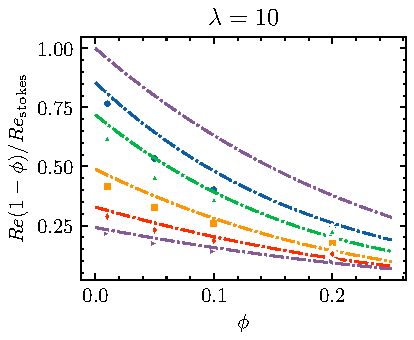
\includegraphics[height = 0.25\textwidth]{image/HOMOGENEOUS_final/CA/U_l_10.pdf}
    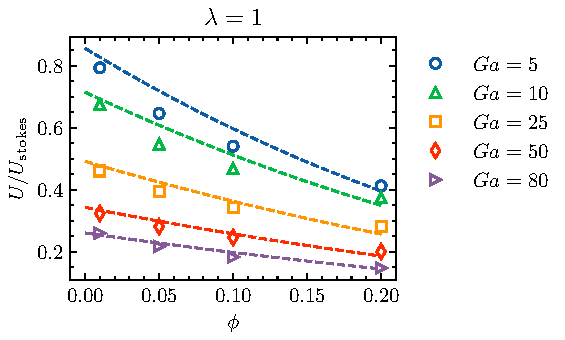
\includegraphics[height = 0.25\textwidth]{image/HOMOGENEOUS_final/CA/U_l_1.pdf}
    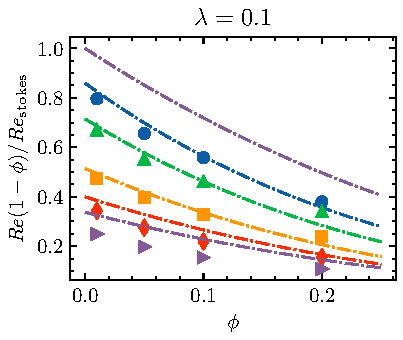
\includegraphics[height = 0.25\textwidth]{image/HOMOGENEOUS_final/CA/U_l_0.pdf}
    \caption{
        Dimensionless rising velocities for (top left) $\lambda  = 10$ (top right) $\lambda =1$ and (bottom) $\lambda = 0.1$. 
        The symbols represents the differents \textit{Galileo} numbers. 
        (dashed lines) Theoretical prediction form \ref{eq:CD0}. 
    }
    \label{fig:drag_force}
\end{figure}



%\subsection{Interphase drag force}
%\subsection{Droplets configurations flowlines and deformations }

\subsection{The Reynolds stress}

Objectives : 
\begin{itemize}
    \item Present the decomposition of the fluid reynolds stress according to isotropic and deviatoric part.
    \item Show the relation between the flowlines graphs and the actual values of the velocity fluctuation.
    \item Compare our case with \citet{almeras2019fluctuations}
\end{itemize}



We decompose both Reynolds stress into an isotropic part and deviatoric part such that, 
\begin{align}
    \bm{\sigma}^{\text{Re}}_p &=  \rho_d \phi_d K^*_p
    \left[
        \textbf{I}(\textbf{u}_p - \textbf{u}_c)\cdot (\textbf{u}_p - \textbf{u}_c) 
        +\textbf{B}_c \cdot (\textbf{u}_p - \textbf{u}_c)(\textbf{u}_p - \textbf{u}_c)
    \right]\\
    \bm{\sigma}^{\text{Re}}_c &=  \rho_c \phi_c K_c^*
    \left[
        \textbf{I}(\textbf{u}_p - \textbf{u}_c)\cdot (\textbf{u}_p - \textbf{u}_c) 
        +\textbf{B}_p \cdot (\textbf{u}_p - \textbf{u}_c)(\textbf{u}_p - \textbf{u}_c)
    \right]
\end{align}
where the $K^*$ is the dimensionless pseudo-turbulent  kinetic energy, $\textbf{I}$ a unit tensor and $\textbf{B}$ a tensor accounting for the deviation of the Reynolds stress left to determine. 

\subsection{The continuous phase Reynolds stress}
\todo{try \citet{almeras2021statistics} fits}
\todo{also check \citet{almeras2019fluctuations} results}
\tb{might be good to plot the velocity field to examine where does the fluctuation arise (pseudo-turbe or turbe)}
Look at \citep{wang2021numerical} and Mahra.. 2015 



The fluid averaged kinetic energy can be easily scaled on the numerical results shown \ref{fig:Tf_Bf}(left).
\begin{figure}[h!]
    \centering
    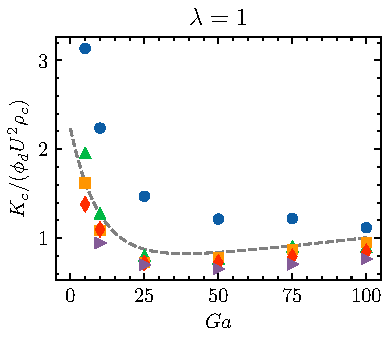
\includegraphics[height=0.3\textwidth]{image/HOMOGENEOUS/fCA/Tf_l_1.pdf}
    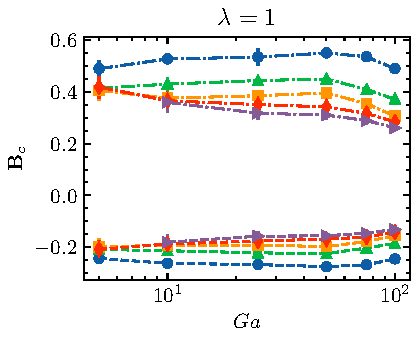
\includegraphics[height=0.3\textwidth]{image/HOMOGENEOUS/fCA/Bf_l_1.pdf}

    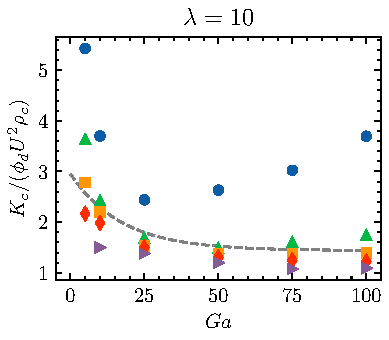
\includegraphics[height=0.3\textwidth]{image/HOMOGENEOUS/fCA/Tf_l_10.pdf}
    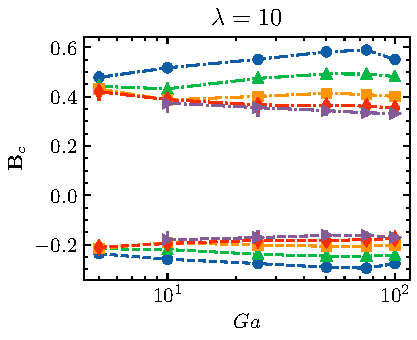
\includegraphics[height=0.3\textwidth]{image/HOMOGENEOUS/fCA/Bf_l_10.pdf}
    \caption{(left) Dimensionless turbulent kinetic energy in terms of the \textit{Galileo} number for different $\phi$. (dots) Numerical simulations, (dashed line) empirical formula \ref{eq:Tf_scaling}.
    The symbols correspond to different volume fraction ($\bullet$) $\phi = 1\%$, ($\blacktriangle$) $\phi = 5\%$, ($\blacksquare$) $\phi = 10\%$, ($\blacklozenge$) $\phi = 15\%$ and ($\blacktriangleright$) $\phi = 20\%$.
    (right) deviatoric part of the Reynolds stress, ($- \cdot -$)  vertical components, $B_{yy}$, ($- -$)  horizontal components, $B_{xx} = B_{zz}$.}
    \label{fig:Tf_Bf}
\end{figure}
\subsection{The particles phase Reynolds stress}

\tb{Maybe include velocity fluctuation and compare to : Lingxin2021 }

\tb{Include Gaussian distribution of bubbles !!! ! ! ! }
Now let's focus on the particular averaged Reynolds stress tensor.
\ref{fig:Talpha_Balpha} shows that the granular temperature behavior is quite similar from the continuous averaged turbulent kinetic energy.
\begin{figure}[h!]
    \centering
    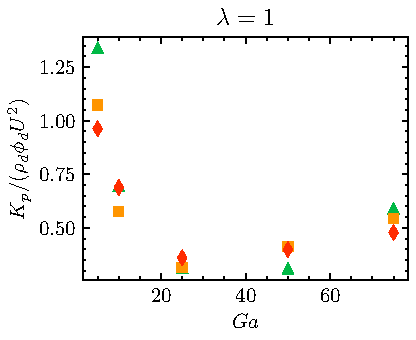
\includegraphics[height=0.3\textwidth]{image/HOMOGENEOUS/fPA/Talpha_l_1.pdf}
    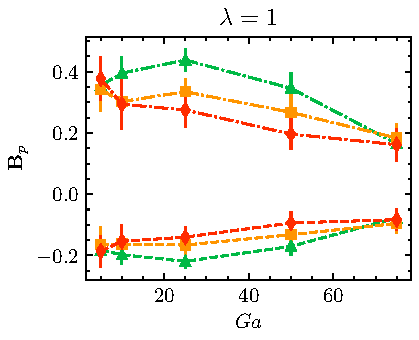
\includegraphics[height=0.3\textwidth]{image/HOMOGENEOUS/fPA/Balpha_l_1.pdf}

    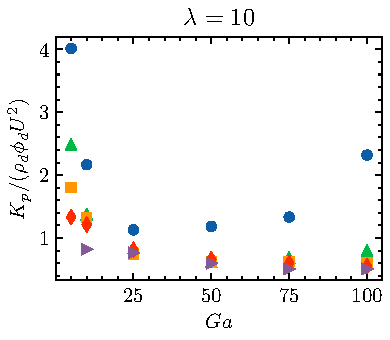
\includegraphics[height=0.3\textwidth]{image/HOMOGENEOUS/fPA/Talpha_l_10.pdf}
    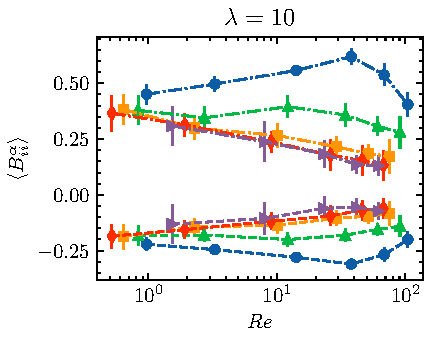
\includegraphics[height=0.3\textwidth]{image/HOMOGENEOUS/fPA/Balpha_l_10.pdf}
    \caption{(left) Dimensionless turbulent kinetic energy in terms of the \textit{Galileo} number for different $\phi$. (dots) Numerical simulations, (dashed line) empirical formula \ref{eq:Talpha_scaling}.
    (right) deviatoric part of the Reynolds stress, ($\bullet$) are the vertical components, $B_{yy}$, ($\blacktriangle$) are the horizontal components, $B_{xx} = B_{zz}$.}
    \label{fig:Talpha_Balpha}
\end{figure}
We can also provide a scaling for the granular temperature, it reads as,  
\begin{equation}
    \frac{\pnavg{T_\alpha}}{U^2}  \approx \frac{\phi}{Ga^2} 2.86\cdot10^{4} 
    \label{eq:Talpha_scaling}
\end{equation}
From \ref{fig:Talpha_Balpha} we observe that this scaling is valid for the lowest \textit{Galileo}. 
The deviatoric part of $\pnavg{T_\alpha}$ is displayed on \ref{fig:Talpha_Balpha}.
It tells us that the Reynolds stress for the particular phase tends to be isotropic in the same way as $\cavg{T}$. 
Indeed, the components of $\pnavg{\textbf{B}}$ go to zero with increasing $Ga$ and $\phi$. 
This behavior is explained by the higher rate of collision present for higher volume fraction and inertia \citep[chapter 1]{jackson2000dynamics}




\section{Nearest particle statistics}







\subsection{Nearest particles arrangements}
\begin{itemize}
    \item Problematic : "How the particles are arranged relative to each other"
    \item Show : "How to compute the Radial and azimuthal probability density function : $P_{nst}(r)$  and $P_{nst}(\theta)$"
    \item  Conclusion on $P_{nst}(\theta)$ : "We observe that the particles pair becomes oriented with increasing $Ga$ and decreasing volume fraction.
    \item  Conclusion on $P_{nst}(r)$ : "We observe that the particles pair becomes randomly arranged for high $Ga$ but in average they are rather spaced from each other" 
\end{itemize}
\tb{Je me demande si cette section est vraiment utile .... car elle n'apport pas d'explication supplementaire a la drag force ni aux fluctuations, c'est peux être mieux de garder ca pour l'article qui traîte des interactions }

In this section we wish to investigate the particle arrangements and clustering effects. 
As in the previous section we treat this problem with the nearest particle statistics.
We introduce the probability density function defined such that $P_{nst}(\textbf{r})d\textbf{r}$ is the probable number of nearest neighboring particle at a disatnce $\textbf{r}$ from a test particle at $\textbf{r} = 0$. 
Let $\textbf{x}^i(t,\CC)$ and $\textbf{x}^j(\CC,t)$ be the position vector of the particle $i$ and $j$ function of the initial configuration of the flow $\CC$ and the time $t$. 
Then, the nearest pair probability density function is defined such as, 
\begin{equation}
    P_{nst}(\textbf{x},\textbf{r},t)= 
    \int \sum_{i}\delta(\textbf{x}-\textbf{x}^i(\CC,t))
    \sum_{j\neq i}\delta(\textbf{x}+\textbf{r}-\textbf{x}^j(\CC,t)) 
    % \delta(t+a-t_c^{ij}(\CC,t)) 
    h_{ij}(\CC,t) d\mathscr{P} 
    \label{eq:P_nstij}
\end{equation}
with $h_{ij} = 1$ if the particle $j$ is one of the nearest neighbor from the particle $i$, and $h_{ij} = 0$ if it is not. 
Since we model a statistically homogeneous configuration within space and time, the variable \textbf{x} and $t$ are of no interest, thus $P_{nst}(\textbf{x},\textbf{r},t) = P_{nst}(\textbf{r})$. 
\begin{figure}
    \centering
    \begin{tikzpicture}
        \node at (0,0){ 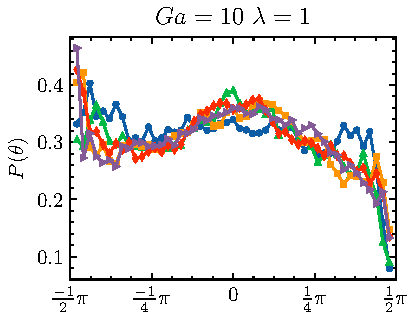
\includegraphics[height=0.3\textwidth]{image/HOMOGENEOUS/fDrop/Pnst_theta_mu_r_1_0_Ga_10.pdf} };
        \node at (0.4\textwidth,0){ 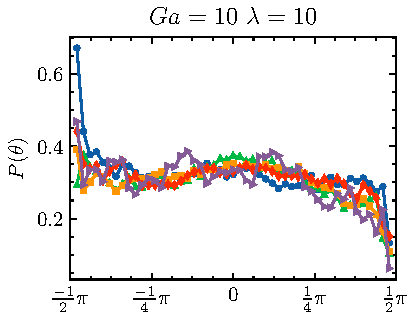
\includegraphics[height=0.3\textwidth]{image/HOMOGENEOUS/fDrop/Pnst_theta_mu_r_0_1_Ga_10.pdf} };
        \node at (0,-0.3\textwidth){ 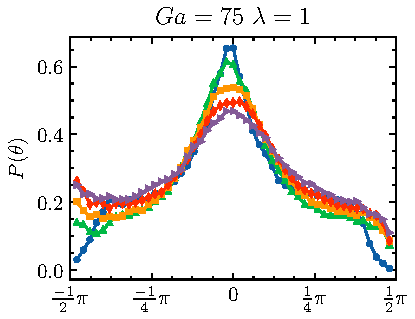
\includegraphics[height=0.3\textwidth]{image/HOMOGENEOUS/fDrop/Pnst_theta_mu_r_1_0_Ga_75.pdf} };
        \node at (0.4\textwidth,-0.3\textwidth){ 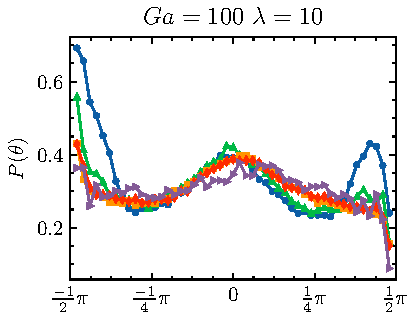
\includegraphics[height=0.3\textwidth]{image/HOMOGENEOUS/fDrop/Pnst_theta_mu_r_0_1_Ga_100.pdf} };
        % \node at (0,-0.6\textwidth){ 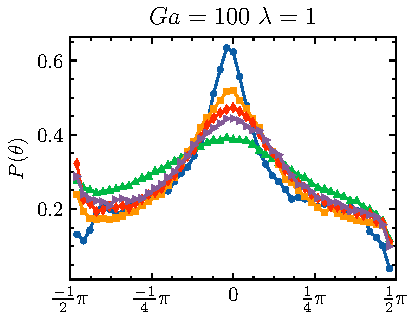
\includegraphics[height=0.3\textwidth]{image/HOMOGENEOUS/fDrop/Pnst_theta_mu_r_1_0_Ga_100.pdf} };
        % \node at (0.4\textwidth,-0.6\textwidth){ 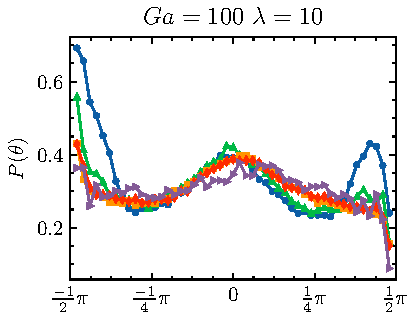
\includegraphics[height=0.3\textwidth]{image/HOMOGENEOUS/fDrop/Pnst_theta_mu_r_0_1_Ga_100.pdf} };
    \end{tikzpicture}
    \caption{Probability density function of the nearest particles : $P_{nst}(\theta)$ for different $Ga$ and $\lambda$. 
    Increasing $Ga$ from top to bottom, (left) $\lambda = 1$ (right) $\lambda = 10$. 
    The symbols correspond to different volume fraction ($\bullet$) $\phi = 1\%$, ($\blacktriangle$) $\phi = 5\%$, ($\blacksquare$) $\phi = 10\%$, ($\blacklozenge$) $\phi = 15\%$ and ($\blacktriangleright$) $\phi = 20\%$.
    (dashed lines) empirical formulas }
    \label{fig:P_nst_theta}
\end{figure}
By using polar coordinate such that $d \textbf{r} = r^2 \sin \phi dr d\phi d\theta$ we can further reduce the PDF to the only consideration of the angular dependency $\theta$ or the distance dependency $r$. 
These reduced p.d.f can be computed as follow, 
\begin{align*}
    P_{nst}(r) 
    &= \int_{-\pi/2}^{\pi/2}\int_{0}^{2\theta} P_{nst}(\textbf{x},\textbf{r},t) \sin \theta  d\phi d\theta\\
    P_{nst}(\theta)
    &= \int_{0}^{\infty}\int_{0}^{2\theta} P_{nst}(\textbf{x},\textbf{r},t) r^2  dr d\phi
\end{align*}
\todo{Check if those formulas are true}
Then $P_{nst}(\theta)$ is the probability that the nearest neighbor of a test particle is inclined at an angle $\theta$ relative to the flow direction. 
We observe that the particles pair becomes oriented with increasing $Ga$ and decreasing volume fraction

On \ref{fig:P_nst_theta} we observe that the particles pair becomes oriented with increasing $Ga$ and decreasing volume fraction.
Indeed, we observe a clear peak of $P_{nst}(\theta)$ at $\theta = \frac{\pi}{2}$. 
It seems that this tendency was also reported for spherical bubble in air-water system \citet{bunner2003effect}. 
Additionally, from \ref{fig:P_nst_theta} we can say that the viscosity ratio $\lambda$ seem to prevent the alignment/clustering of particles denoted by the slightly low peak for $\lambda =10$. 
\todo[inline]{Compart the Orientation with bubbly and solid flows \citet{roghair2011drag}}

\begin{figure}
    \centering
    \begin{tikzpicture}
        \node at (0,0){ 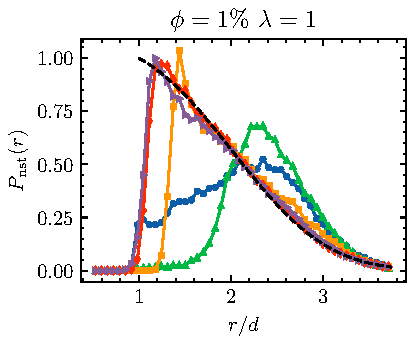
\includegraphics[height=0.3\textwidth]{image/HOMOGENEOUS/fDrop/Pnst_r_mu_r_1_0_PHI_1.pdf} };
        \node at (0.4\textwidth,0){ 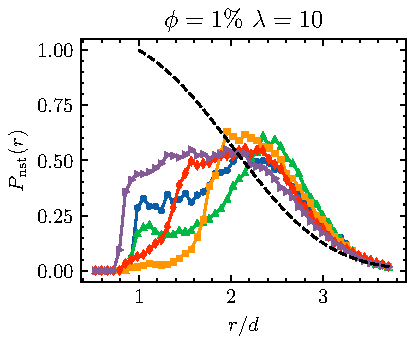
\includegraphics[height=0.3\textwidth]{image/HOMOGENEOUS/fDrop/Pnst_r_mu_r_0_1_PHI_1.pdf} };
        \node at (0,-0.3\textwidth){ 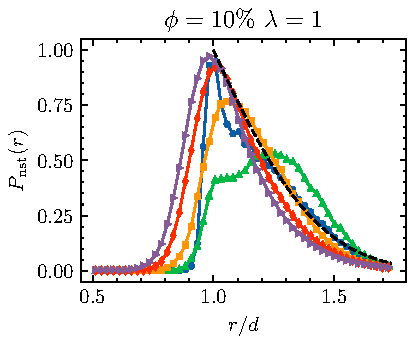
\includegraphics[height=0.3\textwidth]{image/HOMOGENEOUS/fDrop/Pnst_r_mu_r_1_0_PHI_10.pdf} };
        \node at (0.4\textwidth,-0.3\textwidth){ 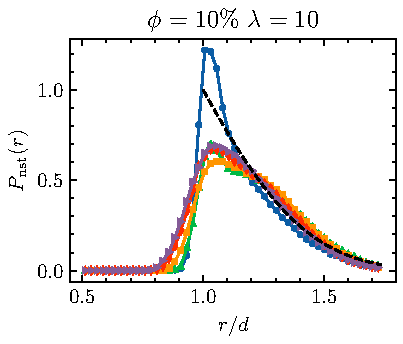
\includegraphics[height=0.3\textwidth]{image/HOMOGENEOUS/fDrop/Pnst_r_mu_r_0_1_PHI_10.pdf} };
        \node at (0,-0.6\textwidth){ 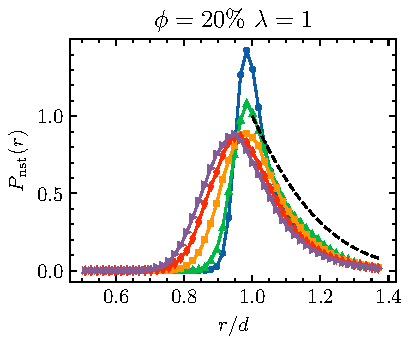
\includegraphics[height=0.3\textwidth]{image/HOMOGENEOUS/fDrop/Pnst_r_mu_r_1_0_PHI_20.pdf} };
        \node at (0.4\textwidth,-0.6\textwidth){ 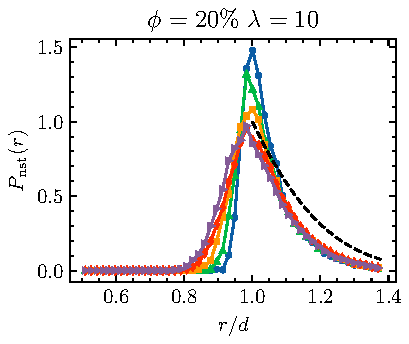
\includegraphics[height=0.3\textwidth]{image/HOMOGENEOUS/fDrop/Pnst_r_mu_r_0_1_PHI_20.pdf} };
    \end{tikzpicture}
    \caption{Radial probability density function : $P_{nst}(r)$ for different $\phi$ and $\lambda$. 
    Increasing $\phi$ from top to bottom, (left) $\lambda = 1$ (right) $\lambda = 10$. 
    The symbols correspond to different Galileo number ($\bullet$) $Ga = 10$, ($\blacktriangle$) $Ga = 25$, ($\blacksquare$) $Ga = 50$, ($\blacklozenge$) $Ga = 75$ and ($\blacktriangleright$) $Ga = 100$.
    (dashed lines) Theoretical formula \ref{eq:P_nst_r}}
    \label{fig:P_nst_r}
\end{figure}
Note that for solid spherical particle in the dilute regime a theoretical formula for $P_{nst}(r)$ can be found assuming completely random distribution and no interactions nor overlap between particles \citep{zhang2021ensemble}, it reads, 
\begin{equation*}
    P_\text{nst}^\text{th}(r) = n_p e^{-4 \pi n_p (r^3 - d^3)/3}.
    \label{eq:P_nst_r}
\end{equation*}
It is evident that all the distribution presented \ref{fig:P_nst_r} have a peak at $r > 1$ where the theoretical formula  predict a peak at $r=1$. 
This is obviously due to the fact that we are in presence of particles interaction which tends to repulse the particles from each others and therefore to shift the distribution to the left. 
What is more interesting is that for $\lambda = 1$ at low volume fraction and high \textit{Galileo} we are able to recover approximately the random particle distribution $P_\text{nst}^\text{th}$ with our numerical results. 
Whereas for $\lambda = 10$ the particle are relatively maintained far from  each other as depicted \ref{fig:P_nst_r}(right). 
We can stipulate that for high viscosity ratio the particles have a tendency to generate more particle fluid mediated interaction as demonstrated by the flow lines \ref{fig:Stream}.


\subsection{Nearest-particle average fluid velocity}
Objectives : 
\begin{itemize}
    \item Problematic "How to analyse the flow around a particle in average"
    \item First : present the averaged the nearest particles' statistics method. And how to compute the nearest averaged velocity fields $\nstavg{\textbf{u}}$.
    \item Present the flowlines and show that for $\phi = 5 \rightarrow 20\%$ we observe that a vertical symmetry arise.
    \item Explain how this field it is related to the velocity fluctuation with \ref{eq:def_uu}
    \item Conclude that these velocity fields represent the PWFs since it represent the mean wakes \citep{du2022analysis}.  
    \item Additionally, some comment can be made regarding the shape of the particle thanks to the contour lines. 
    \item Approach these flow fields by analytical solution of potential flow to obtain an analytical solution for teh reyolds stress. 
\end{itemize}

Presently, we wish to investigate the  averaged flow structure around a fluid particle.
To obtain such a field we make use of the nearest particle statistics recently introduced by \citet{zhang2021stress}. 
We introduce $\nstavg{\textbf{u}}(\textbf{x},\textbf{r})$ as the velocity fields at \textbf{x} knowing there is a particles center of mass located at \textbf{r}.
Additionally, this particle is the nearest particle among all to the point \textbf{x}.  
Formally, this conditional average can be written as, 
\begin{equation}
    \nstavg{\textbf{u}}(\textbf{x},\textbf{r})=\frac{1}{P_{nst}(\textbf{x},\textbf{r})} 
    \int \textbf{u}(\textbf{x},\CC,t) 
    \sum_{\alpha}\delta(\textbf{x}+\textbf{r}-\textbf{x}^\alpha(\CC,t)) h_{\alpha}(\CC,\textbf{x},t) d\mathscr{P} 
    \label{eq:q_nst_avg}
\end{equation}
where $P_{nst}(\textbf{x},\textbf{r})$ is defined as,  
\begin{equation}
    P_{nst}(\textbf{x},\textbf{r})= 
    \int
    \sum_{\alpha}\delta(\textbf{x}+\textbf{r}-\textbf{x}^\alpha(\CC,t)) 
    h_\alpha(\CC,\textbf{x},t) d\mathscr{P}. 
    \label{eq:P_nsti}
\end{equation}
which is the probability of finding a particle center of mass at a distance \textbf{r} from the point \textbf{x} knowing that this particle is the nearest neighbor to the points \textbf{x}. 
The function $h_\alpha$ is defined such that, $h_\alpha = 1/N^p$ if $\alpha$ is the nearest particle to \textbf{x} and $0$ if not, where $N^p$ is the total number of nearest neighbor.
Indeed, the point \textbf{x} at mid-distance from two particles posses two nearest neighbors by definition, thus $N(\textbf{x},\CC,t) = 2$ in this case. 

\todo[inline]{Include the numerical computaiton of $\nstavg{\textbf{u}}$.  }

\ref{fig:Stream} shows the streamline of the field $\nstavg{\textbf{u}}(\textbf{x},\textbf{r})$ for three volume fractions. 
We clearly observe the induced wake of the particles centered at the origin. 

\begin{figure}
    \centering
    \begin{tikzpicture}
        \node (img) at (0,0)  {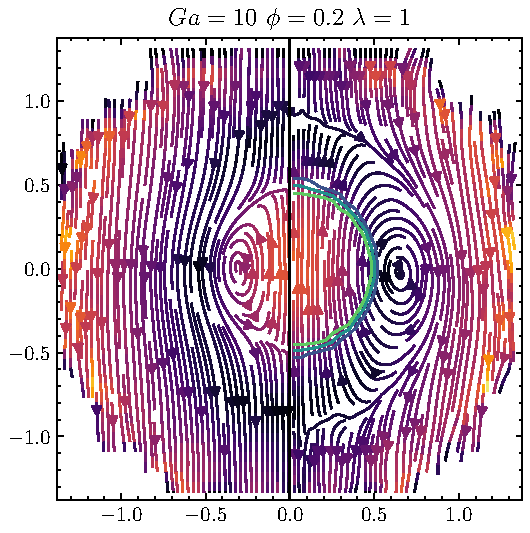
\includegraphics[height=0.4\textwidth]{image/VALIDATION2.0/Stream/Stream_PHI_20_Ga_10_l_1.pdf}};
        \node (img) at (0.4\textwidth,0)  {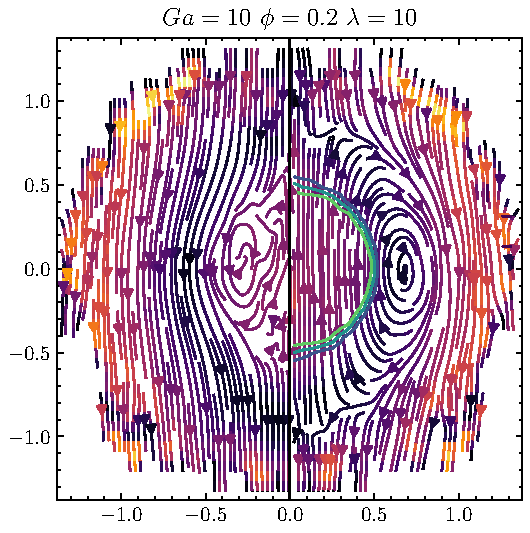
\includegraphics[height=0.4\textwidth]{image/VALIDATION2.0/Stream/Stream_PHI_20_Ga_10_l_10.pdf}};
        \node (img) at (0,-0.4\textwidth)  {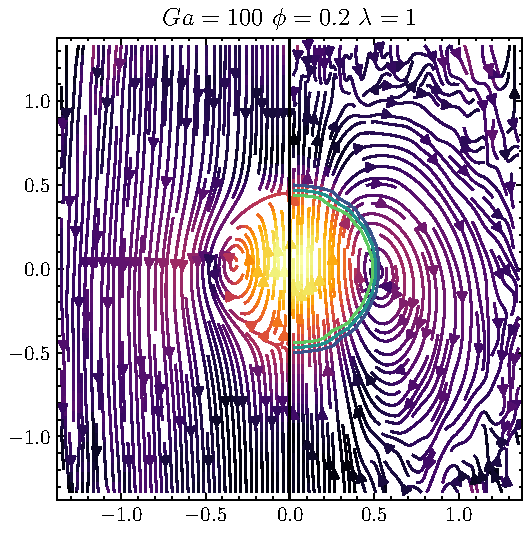
\includegraphics[height=0.4\textwidth]{image/VALIDATION2.0/Stream/Stream_PHI_20_Ga_100_l_1.pdf}};
        \node (img) at (0.4\textwidth,-0.4\textwidth)  {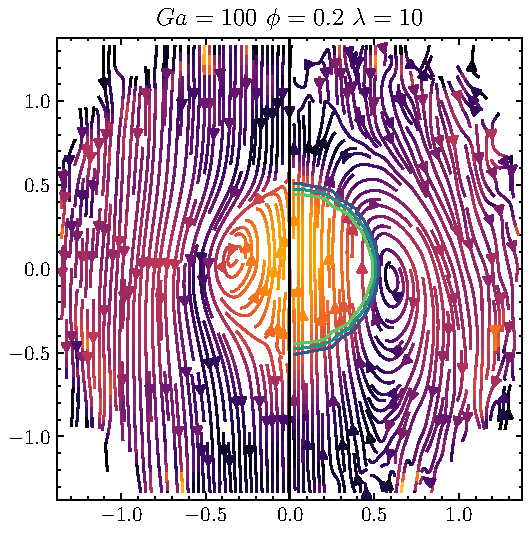
\includegraphics[height=0.4\textwidth]{image/VALIDATION2.0/Stream/Stream_PHI_20_Ga_100_l_10.pdf}};
        \node (img) at (0,-0.8\textwidth)  {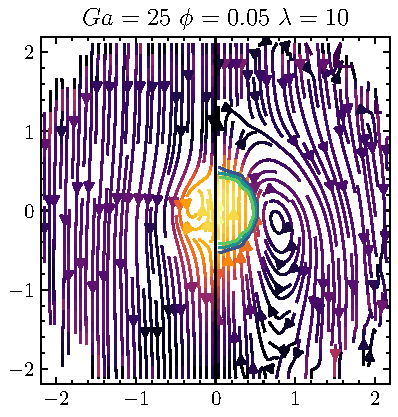
\includegraphics[height=0.4\textwidth]{image/VALIDATION2.0/Stream/Stream_PHI_5_Ga_25_l_10.pdf}};
        \node (img) at (0.4\textwidth,-0.8\textwidth)  {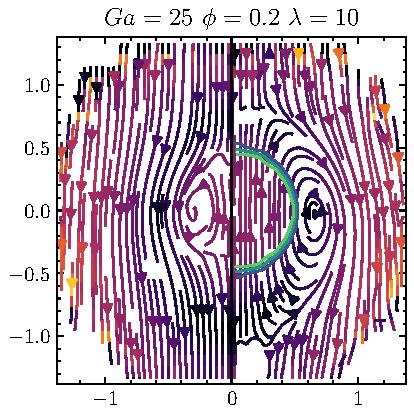
\includegraphics[height=0.4\textwidth]{image/VALIDATION2.0/Stream/Stream_PHI_20_Ga_25_l_10.pdf}};
    \end{tikzpicture}
    \caption{Nearest particle averaged velocity $\nstavg{\textbf{u}}(\textbf{r})$ for  $\phi = 5\%$ and $20\%$.
    Green lines : contour plots of the nearest averaged indicator function $\nstavg{\chi_d}(\textbf{r})$ (it represent the mean shape of the particles)}
    \label{fig:Stream}
\end{figure}
It is evident from these plots that the induced wake is the averaged wake resulting from the averaged translation of the particles. 
And this averaged wake has a tendency to be asymmetrical for low volume fraction and symmetrical for higher ones. 
Additionally, form basic mathematical consideration on the average operators we can demonstrate that :
\begin{multline*}
    \avg{\chi_k \textbf{u}'_k\textbf{u}'_k}(\textbf{x},t)
    + \phi_k \textbf{u}_k\textbf{u}_k
    = \\
    \underbrace{\int (\nstavg{\chi_k \textbf{u}^0_k}  \nstavg{\chi_k \textbf{u}^0_k} / (\nstavg{\chi_k})  P_{nst}(\textbf{x},t,\textbf{r}) d\textbf{r} }_\text{PWFs}
    +\underbrace{\int \nstavg{\chi_k \textbf{v}_k^0\textbf{v}_k^0}  P_{nst}(\textbf{x},t,\textbf{r}) d\textbf{r}}_\text{WIA}
    \label{eq:def_uu}
\end{multline*}
where, $\textbf{v}_k^0  = \textbf{u}_k^0 - \nstavg{\chi_k \textbf{u}^0_k} / \nstavg{\chi_k}$ is the fluctuation of the local velocity relative to the nearest averaged value. 
Consequently, we can decompose the ensemble averaged fluid velocity fluctuations with a first term representing the variance of $\nstavg{\textbf{u}}$ around the mean $\textbf{u}_k$, and a second term representing the variance of $\textbf{u}^0_k$ around the mean  $\nstavg{\textbf{u}}$. 

There are two phenomena causing velocity fluctuations in the liquid:
the agitation resulting from wakes and their collective interactions [wake-induced agitation (WIA)], and the non-turbulent fluctuations resulting from averaged wakes and potential flows around bubbles [potential flow and averaged wake fluctuations (PWFs)].
As a matter of fact in the phase space of $\nstavg{\textbf{u}}(\textbf{r})$ the bubble is fixed at the origin thus we recover the velocity fields representing what is called the PWFs. 
In their study \citet{du2022analysis} carry out transient simulation with fixed particles to recover the PWFs components here we show that a single simulation permit us to recover WIA and PWFs by the mean of the nearest particles' statistics. 

\todo[inline]{make the link with drag force/drag coef  \citet{dandy1989buoyancy}}
\todo[inline]{make the link with velocity fluctuation \citet{almeras2021statistics}}








% \subsection{The particle-fluid-particle Stress}
\begin{figure}
    \centering
    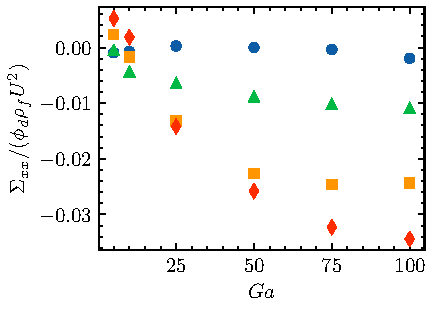
\includegraphics[height=0.3\textwidth]{image/HOMOGENEOUS/fPA/PFPxx.pdf}
    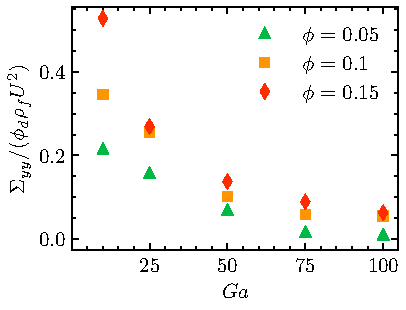
\includegraphics[height=0.3\textwidth]{image/HOMOGENEOUS/fPA/PFPyy.pdf}
    \caption{(left) Normalized PFP stress }
\end{figure}

Open the discussion on the fact that we yet still not have enought data for the pfp stress
% 
\subsection{Higher moments closure : Stresslet ? ? }


\begin{equation}
    \ddt \mathcal{P}_\alpha
    = \int_{\Omega_\alpha} \left(
        \rho_2  \textbf{w}_2 \textbf{w}_2 
        + \textbf{r} \nablab \cdot \mathbf{T}_2
    \right) d\Omega
\end{equation}
\begin{equation}
    \ddt \mathcal{P}_\alpha
    = \int_{\Omega_\alpha} \left(
        \rho_2  \textbf{w}_2 \textbf{w}_2 
        + \mathbf{T}_2
    \right) d\Omega
+ \int_{\Sigma}\textbf{rT}_2 \cdot \textbf{n}_2 d\Sigma
\end{equation}
surface jump condition : 
\begin{equation}
    - \int_{\Sigma_\alpha} 
    \sigma \textbf{I}_{||}
d\Sigma
= \int_{\Sigma}\textbf{rT}_1 \cdot \textbf{n}_1 d\Sigma
+ \int_{\Sigma}\textbf{rT}_2 \cdot \textbf{n}_2 d\Sigma
\end{equation}
\begin{equation}
    \ddt \mathcal{P}_\alpha
    = \int_{\Omega_\alpha} \left(
        \rho_2  \textbf{w}_2 \textbf{w}_2 
        - \mathbf{T}_2
    \right) d\Omega
    - \int_{\Sigma_\alpha} 
        \sigma \textbf{I}_{||}
    d\Sigma
    + \int_{\Sigma}\textbf{rT}_1 \cdot \textbf{n}_2 d\Sigma
\end{equation}
\begin{figure}[h!]
    \centering
    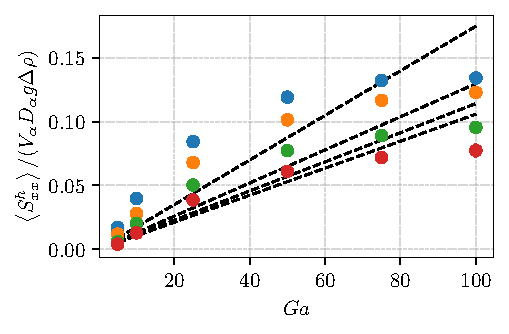
\includegraphics[height=0.3\textwidth]{image/HOMOGENEOUS/fPA/Sxx.pdf}
    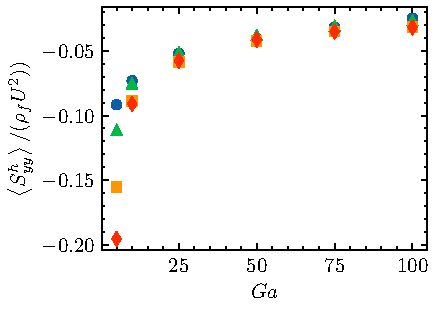
\includegraphics[height=0.3\textwidth]{image/HOMOGENEOUS/fPA/Syy.pdf}
\end{figure}
\begin{equation}
    \int_{\Sigma}\textbf{r}_1 (\textbf{T}_1  -  \oneavg{\textbf{T}_1}) \cdot \textbf{n}_2 d\Sigma
    = \int_{\Omega_\alpha} \left(
        \mathbf{T}_2
        - \rho_2  \textbf{w}_2 \textbf{w}_2 
    \right) d\Omega
     + \int_{\Sigma_\alpha} 
     \sigma \textbf{I}_{||}
    d\Sigma
    + \ddt \mathcal{P}_\alpha
    -\int_{\Sigma}\textbf{r}_1   \oneavg{\textbf{T}_1} \cdot \textbf{n}_2 d\Sigma
\end{equation}
Assuming that $\textbf{T}_k = - p_k \textbf{I} + \mu_k \mathbb{S}_k  = -p_k \textbf{I} + \mu_k (\nablab \textbf{u}_k + \nablab \textbf{u}_k^T )$ 
\begin{multline}
    \int_{\Sigma}\textbf{r}_1 (\textbf{T}_1  -  \oneavg{\textbf{T}_1}) \cdot \textbf{n}_2 d\Sigma
    \\= \dot{ \mathcal{P}_\alpha}
    + \int_{\Omega_\alpha} \left(
        \mu_2\mathbb{S}_2
        - \rho_2  \textbf{w}_2 \textbf{w}_2 
    \right) d\Omega
     + \int_{\Sigma_\alpha} 
     \sigma \textbf{I}_{||}
    d\Sigma
    - \textbf{I} \int_{\Omega_\alpha} p_2 d\Omega
    + v_\alpha \oneavg{p}
    - \mu_1 v_\alpha \oneavg{\mathbb S}
\end{multline}
\begin{multline}
    \int_{\Sigma}\textbf{r}_1 (\textbf{T}_1  -  \oneavg{\textbf{T}_1}) \cdot \textbf{n}_2 d\Sigma
    \\= \dot{ \mathcal{P}_\alpha}
    + \int_{\Omega_\alpha} \left(
        \mu_2\mathbb{S}_2
        - \rho_2  \textbf{w}_2 \textbf{w}_2 
    \right) d\Omega
     + \int_{\Sigma_\alpha} 
     \sigma \textbf{I}_{||}
    d\Sigma
    - \textbf{I} \int_{\Omega_\alpha} p_2 d\Omega
    + v_\alpha \oneavg{p}
    - \mu_1 v_\alpha \oneavg{\mathbb S}
\end{multline}
Keeping only  the deviatoric part of the equations
\begin{equation}
    \textbf{S}_\alpha
    = \dot{ \mathcal{P}_\alpha}
    + \int_{\Omega_\alpha} \left(
        \mu_2\mathbb{S}_2
        - \rho_2  \textbf{w}_2 \textbf{w}_2 + w^2_2/3
    \right) d\Omega
     + \int_{\Sigma_\alpha} 
     \sigma \textbf{I}_{||}^{dev}
    d\Sigma
    - \mu_1 v_\alpha \oneavg{\mathbb S}
\end{equation}
For an almost spherical drop in a stokes regime: 
\begin{equation}
    \textbf{S}_\alpha
    = 
    \int_{\Omega_\alpha} \left(
        \mu_2\mathbb{S}_2
    \right) d\Omega
    - \mu_1 v_\alpha \oneavg{\mathbb S}
\end{equation}
 
The original formulas stipulate that :

\todo{This formulation must be chnaged look at \citet[chap 5]{pozrikidis1992boundary}}
\begin{align}
    \label{eq:M_decomposition}
    S^\alpha_{ij} 
    &= \frac{1}{2}  \int_{\Sigma_\alpha} \left[
        r_i(T_{jk}n_k)
        + (T_{ik}n_k)r_j
        \right]d\Sigma
        - \frac{\delta_{ij}}{3}\int_{\Sigma_\alpha} \left[
            r_l(T_{lk}n_k)
    \right]d\Sigma
    -\mu_1 \int_{\Sigma_{\alpha}}
    (u_in_j^2 + u_jn_i^2)d\Sigma
    \\
    T^\alpha_{ij}
    &= \frac{1}{2}  \int_{\Sigma_\alpha} \left[
        r_i(T_{jk}n_k)
        - (T_{ik}n_k)r_j
    \right]d\Sigma \nonumber
\end{align}

Inter changing the sens of the normal vector we can rewrite the last term of \ref{eq:M_decomposition} such as :
\begin{align}
    - \mu_1 \int_{\Sigma_{\alpha}}
    (u_in_j + u_jn_i)d\Sigma
    = 
    + \mu_1 \int_{\Sigma_{\alpha}}
    (u_i n^1_j + u_jn^1_i)d\Sigma
\end{align}
Using Gauss divergence theorem 
\begin{align}
    - \mu_1 \int_{\Sigma_{\alpha}}
    (u_in_j + u_jn_i)d\Sigma
    = 
    \mu_1 \int_{\Omega_1}
    (\nablab u_i + \nablab u_j )d\Omega
\end{align}
which correspond the average of the continuous phase stress in homogeneous medium.
Besides in Stokes flows :
\begin{equation}
    \frac{1}{2}  \int_{\Sigma_\alpha} \left[
        r_i(T_{jk}n_k)
        + (T_{ik}n_k)r_j
        \right]d\Sigma
    =
    \frac{1}{2}  \int_{\Sigma_\alpha} \left[
        T_{ij}
        + T_{ji}
        \right]d\Sigma
\end{equation}
And so on for the trace, Thus we can rewrite the stresslet as : 


%%%%%%%%%%%%%%%%%%%%%%%%%%%%%%%%%%%%%%%%%%%%%%%%
%%%%%%%%%%%%%%%%%%%%%%%%%%%%%%%%%%%%%%%%%%%%%%%%

\section{Conclusion}
We provided statistically representative results for two closure terms and introduce an original numerical methodology.

\section*{Acknowledgement}

\appendix
\section{Statistical convergence and mesh independence studies}
\label{ap:A}
\section{Mesh definition convergence}
\label{ap:convergence}

% \subsection{Statistical and mesh independence study}

In the aim of providing accurate closure terms, it is of primary importance to verify the well convergence of the mean quantities, by varying the mesh definition. 
While the domain size and duration of simulation have been validated in \citet{fintzi2024buoyancy}.
To tackle this problem we carried out four simulations with $125$ rising droplets with different mesh definitions. 
The flow parameters read as,  
\begin{align*}
    \lambda = 10,
    && \zeta = 0.9,
    && Bo = 0.5,
    && Ga = 80,
    && \phi = 0.1,
\end{align*}

\ref{fig:Re_and_Tc}(left) displays the cumulative mean of the vertical Reynolds number based on the drift velocity, namely,
\begin{equation}
    \widetilde{Re}(t)
    = \frac{\rho_f d}{\mu_f t}\int_{t_0}^{t_0+t} \left(\Xavg{\textbf{u}^0_d} -  \Xavg{\textbf{u}_f^0}\right)dt'
\end{equation}
where $t_0$ is the starting sampling time. 
We reach mesh independent results for $d/\Delta \geq 25$ in agreement with the recent studies of \citet{hidman2023assessing} \citet{zhang2021direct} for low inertial bubbly flows.
Also, it is seen that $\widetilde{Re}$ reaches a constant value from $t^* = 50$ to the end of the simulation. 
\begin{figure}[h!]
    \centering
    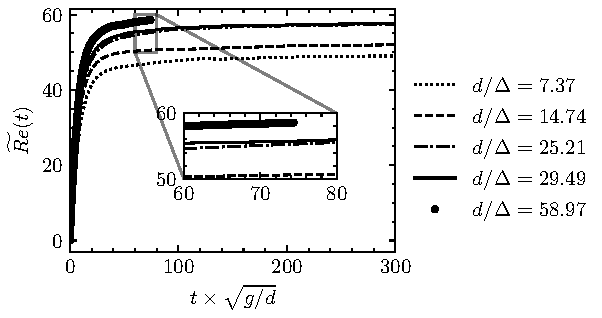
\includegraphics[height = 0.35\textwidth]{image/HOMOGENEOUS_final/CA/Re.pdf}
    \caption{(left) Cumulative mean of the volume averaged Reynolds number along the simulation time based on the drift velocity $U = \textbf{u}_p - \textbf{u}_c$.
    (right) Cumulative mean of the fluid Reynolds stress tesor. }
    \label{fig:Re_and_Tc}
\end{figure}

% The well convergence of the rising velocity doesn't guarantee a statistical nor a mesh convergence for finer quantities such as the pseudo-turbulent kinetic energy. 
% Therefore, we provide on \ref{fig:UpUp} (left) the running average of the fluid phase pseudo-turbulent energy. 
% Similarly, \ref{fig:UpUp} (right) represent the particle center of mass pseudo-turbulent kinetic energy. 
% \begin{figure}[h!]
%     \centering
%     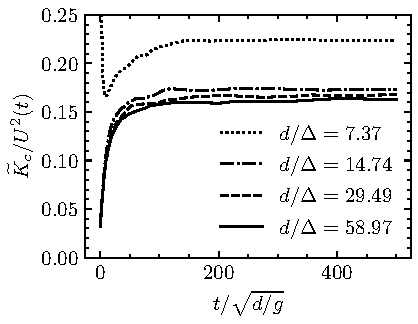
\includegraphics[height = 0.35\textwidth]{image/VALIDATION2.0/fCA/Tcum.pdf}
%     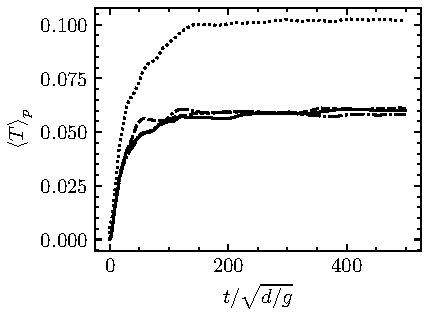
\includegraphics[height = 0.35\textwidth]{image/VALIDATION2.0/fPA/Tcum.pdf}
%     \caption{(left) Cumulative mean of the volume averaged granular temperature along the simulation time based on the drift velocity $U = \textbf{u}_p - \textbf{u}_c$, with $\phi = 0.1$, $\rho_r = 1.11$, $ \mu_r =0.1$ and $Ga = 29.9$ and $N_b = 125$.
%     (right) Cumulative mean of the dimensionless particle-fluid-particle stress horizontal component tensor. }
%     \label{fig:UpUp}
% \end{figure}
% Both figure exhibit well converged data. 
% Interestingly, $\widetilde{K}_c$ and $\widetilde{K}_\alpha$ reach a constant value at $t^* = 200$ which is four time greater than for $\widetilde{Re}$.


% \tb{Cite and compare to Berner and \citet{bunner2002dynamics} which found that Nb > 12 is sufficient \citet{roghair2011drag}}
% Now, let's investigate the required number of droplets per domain, $N_b$, and the minimum definition of cells per diameter of droplets $\delta$.  
% \tb{Include bibliography and expectation here \ldots}
% For this investigation we kept the physical parameters presented in the same section and made a double parametric analysis over $N$ and $\delta$. 
% We carried out simulations for $N = 2, 3, 4, 5, 6, 7$, and for a number of cells $10 <\delta < 40$. 
% In Basilisk the mesh definition is defined by a power of two, consequently depending on the size of the domain (which is fixed to keep a $\phi$ constant) the $\delta$ parameter is fixed at a power of 2 close. 
% \begin{figure}[h!]
%     \centering
%     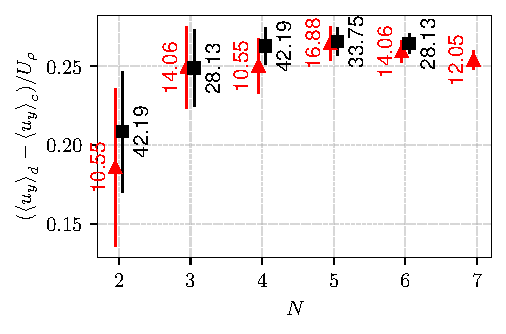
\includegraphics[height= 0.3\textwidth]{image/VALIDATION/N_and_delta/DUd.pdf}
%     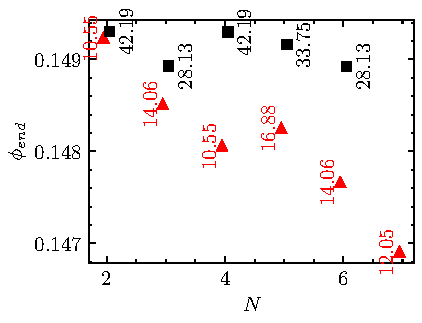
\includegraphics[height= 0.3\textwidth]{image/VALIDATION/N_and_delta/PHI.pdf}
%     \caption{(left) Averaged Reynolds number based on the drift velocity.
%             (right) Dispersed phase volume fraction at the end of each simulation.
%             The text on the side of the points is $\delta$.
%             N correspond to $N = N_b^3$. }
%     \label{fig:VALIDATION_Nd_1}
% \end{figure}
% \ref{fig:VALIDATION_Nd_1}(left), illustrate clearly that the drift velocity is independent of the parameters $N_b$ and $\delta$, for $N >4$. 
% On the other hand, \ref{fig:VALIDATION_Nd_1}(right), show that the volume fraction of the dispersed phase is lower for the low defined grid (red dots), due to a loss of volume during the simulation.
% This doesn't mean that the solver isn't volume conservative. 
% In fact, it is fund to be due to the \href{http://basilisk.fr/sandbox/fintzin/Rising-Suspension/no-coalescence.h}{no-coalescence.h} which generate fragment into the numerical domain, fragment which are deleted in the long run. 
% \begin{figure}[h!]
%     \centering
%     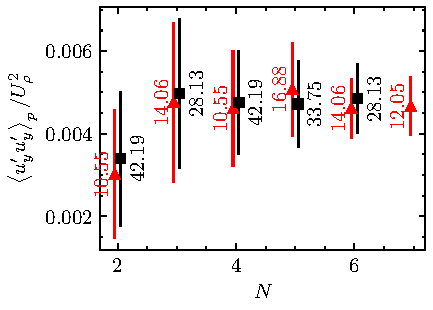
\includegraphics[height= 0.3\textwidth]{image/VALIDATION/N_and_delta/PA_UpUp.pdf}
%     \includegraphics[height= 0.3\textwidth]{image/VALIDATION/N_and_delta/Mh.pdf}
%     \caption{(left) Fluids phase averaged fluctuation tensor.
%             (right) Particular average of the first moment tensor, where $F_g$ is the buoyancy force applied on one droplet. 
%             The numerical values displayed alongside the dots are the number of cells per diameter.}
%     \label{fig:VALIDATION_Nd_2}
% \end{figure}
% Now, let's look at the behavior of more \textit{complicated} closure terms. 
% \ref{fig:VALIDATION_Nd_2}(left) demonstrate that the vertical component of the pseudo turbulent tensor is parameter independent rather early, independently of the grid definition. 
% This fact is rather surprising but note that the standard deviation is quite high for small domain. 
% On \ref{fig:VALIDATION_Nd_2}(right), we can examine the vertical component of the first moment closure term. 
% It is found to be constant for all $N$, but rather inaccurate for coarse grids. 
% Which makes sens since the first moment results from a local calculation of the stress over a droplet volume, unlike the other quantities which results from the averaged center of mass velocity of a droplet. 

% As we have shown, the quantities presented converge for a number of droplets equivalent to $N = 4$ and $\delta = 25$. 
% Thus, we validate our simulation in space, i.e. we made sure that our domain were wide enough to minimize the influence of the periodicity on our results, and in mesh definition. 
% Nevertheless, at it is the number of realization that matter when carrying a particular average, it is interesting to look at the duration of the simulation.



\section{Ordered array of particles}

Following the strategy of \citet{loisy} This appendix treat the case of ordered array of particles. 

Eventhrougth not realistic, the advantage is that in these simulations we do not have any particle-particle interaction.
It is therefore of a great interest to evaluate different properties knowing that 
\begin{figure}[h!]
    \centering    
    \includegraphics[height = 0.35\textwidth]{image/HOMOGENEOUS/fCA/Tf_N_1_l_1.pdf}
    \includegraphics[height = 0.35\textwidth]{image/HOMOGENEOUS/fCA/Tf_N_1_l_10.pdf}

    \includegraphics[height = 0.35\textwidth]{image/HOMOGENEOUS/fCA/Bf_N_1_l_1.pdf}
    \includegraphics[height = 0.35\textwidth]{image/HOMOGENEOUS/fCA/Bf_N_1_l_10.pdf}

    \includegraphics[height = 0.35\textwidth]{image/HOMOGENEOUS/fCA/Cp_N_1_l_1.pdf}
    \includegraphics[height = 0.35\textwidth]{image/HOMOGENEOUS/fCA/Cp_N_1_l_10.pdf}
    \caption{
        (top) dimensionless fluid pseudo turbulent energy. 
        (middle) deviatoric components of the matic B
        (bottom) 
        Drag coefficient and dimensionless force for ordered array. 
        (--) Empirical formula of Rvikind and Ryskin (1976)
        The symbols correspond to different volume fraction ($\blacktriangleleft$) $\phi = 0.1$\%, ($\bullet$) $\phi = 1\%$, ($\blacktriangle$) $\phi = 5\%$, ($\blacksquare$) $\phi = 10\%$, ($\blacklozenge$) $\phi = 15\%$, and ($\blacktriangleright$) $\phi = 20$\%.
    }
    \label{fig:Cp}
\end{figure}


On \ref{fig:Cp}(bottom) we can see that the formula of Rvikind and Ryskin (1976) is valid only in the low inertial regime which is probably due to the wake of the particles in tri periodic domain. Pseudo_turb/Ordered.tex
\section{Shape of the particles}
\label{app:shape}

%\begin{itemize}
%    \item Problematic : "What is teh mean shape of our particles ? "
%    \item Present the definition of the aspect ratio.
%    \item Show how it behaves in terms of $\phi,\lambda$ and $Ga$
%    \item Overall, show that the particles are rather spherical which were also demonstrated by the previous plots regarding the flow lines. 
%    \item Besides the deformation increase with increasing $Ga$ and small $\phi$ which agree with \citet{loisy2017buoyancy}. 
%\end{itemize}


%It is known since \todo{biblio} \citet{bunner2003effect} that droplets or bubbles mean rising velocity is mainly dependent on their shapes. 
%For spherical bubbles it was observed that the rising velocity $Re$ were proportional to $\sim Re_{\phi=0}(1 - \phi^{1/3})$, where $Re_{\phi=0}$ is the isolated rising Reynolds number. 
%Whereas deformable bubbles a $\sim Re_{\phi=0}(1 - \phi)^{3}$ dependency is observed \todo{biblio}. 
%This is n=in fact due to the different arrangement taken by the particles as a consequence of their deformations. 
%Therefore, in order to develop a coherent model we first investigate the droplets mean shapes. 
%After what we present the dependency of the rising velocity and drag force with the main parameters of the problems.  

%The shape of fluid particles has a strong effect on their mean rise velocity. 

%High Bond number bubbles or drops are known to deform significatively. Those deformations have a non-negligible effect on their rise velocity \citep{bunner2003effect,tripathi2014}. In this appendix, we evaluate the deformation of the fluid inclusion within the prescribed range of dimensionless parameters and show that for the whole range of dimensionless parameters, it remains small. Axisymmetric fluid inclusion are characterized by their aspect ratio which is the ratio of their cross-stream axis, to the axis parallel to their velocity. For three-dimensional configuration with deforming fluid inclusion it is not possible to define the aspect ratio as in the axisymmetric configuration since the deformation are not symmetric anymore \citep{bunner2003effect}.  Hence to investigate the shape of each particle we define the inertia tensor for each particle $\alpha$ as

%Bubbles and drops with a substantial Bond number are known to undergo noticeable deformations, and these deformations can significantly influence their upward velocity \citep{bunner2003effect, tripathi2014}. In this appendix, we assess the deformation of fluid inclusions across a specified range of dimensionless parameters. Our findings demonstrate that, within this parameter range, deformations remain consistently small.

%Axisymmetric fluid inclusions are uniquely identified by their aspect ratio—the ratio of their cross-stream axis to the axis parallel to their velocity. However, for three-dimensional configurations involving deforming fluid inclusions, the symmetric nature of deformation is lost \citep{bunner2003effect}. Consequently, the definition of aspect ratio becomes untenable. To explore the shapes of individual particles, we introduce the inertia tensor for each particle $\alpha."

%Bubbles or droplets with a high Bond number are recognized for undergoing significant deformations, and these deformations notably impact their ascent velocity \citep{bunner2003effect,tripathi2014}. This appendix is dedicated to assessing the deformation of fluid inclusions within a specified range of dimensionless parameters. It is demonstrated that, across this entire range, the deformations remain consistently small.

%Axisymmetric fluid inclusions are distinguished by their aspect ratio, defined as the ratio of their cross-stream axis to the axis parallel to their velocity. However, for three-dimensional configurations involving deforming fluid inclusions, the definition of the aspect ratio becomes impractical due to the loss of symmetry in deformations \citep{bunner2003effect}. Consequently, to examine the shape of each particle, we introduce the inertia tensor for each particle, denoted by $\alpha$.


Bubbles or droplets with a high Bond number are known to undergo significant deformations, and these deformations can significantly influence their rising velocity \citep{bunner2003effect,tripathi2014}. This appendix is dedicated to assessing the deformation of fluid inclusions within the range of dimensionless parameters prescribed in the main-body of the article. It is demonstrated that, across this entire range, the deformations remain small. Axisymmetric fluid inclusions are characterized by their aspect ratio, defined as the ratio of their cross-stream axis to the axis parallel to their velocity. However, for three-dimensional configurations involving deforming fluid inclusions, the definition of the aspect ratio becomes impractical due to the loss of symmetry in deformations \citep{bunner2003effect}. Consequently, to examine the shape of each particle, we introduce the inertia tensor for each particle, denoted by $\alpha$.



%Since the drops change orientation with time it is not possible

\begin{equation*}
    \mathcal{I}^\alpha
    = \int_{V_\alpha} \left[
        (\textbf{r}\cdot \textbf{r}) \textbf{I}  - \textbf{rr}
        \right]
    dV.
\end{equation*}

where, \textbf{I} is the identity tensor and $\textbf{r} = \textbf{x} - \textbf{x}_\alpha$. $\textbf{x}_\alpha$ is the centre of mass of the fluid inclusion. \ref{fig:chi} display the averaged aspect ratio of the droplets. Rather than consider all the components of the inertia tensor, we define the mean "aspect ratio" $\chi$ of the particle as 
%It is defined using the conventional manner \citep{bunner2003effect}, namely,
\begin{equation}
    \chi = \pavg{\sqrt{\mathcal{I}_{max}^\alpha /\mathcal{I}_{min}^\alpha} }
\end{equation} 
where $\mathcal{I}_{max}^\alpha$ and $\mathcal{I}_{min}^\alpha$ are the maximum and minimum eigenvalues value of the particle inertia tensor. This definition has been used to characterise the deformation and orientation of rising bubbles \citep{bunner2003effect}. 


\begin{figure}[h!]
    \centering
    \includegraphics[height = 0.35\textwidth]{image/HOMOGENEOUS/fPA/chi_mu_r_1-0.pdf}
    \includegraphics[height = 0.35\textwidth]{image/HOMOGENEOUS/fPA/chi_mu_r_0-1.pdf}
    \caption{Mean aspect ratio of the droplets $\avg{\chi}$ as a function of the \textit{Galileo} number, and the volume faction $\phi$,  for two different viscosity ratios.  
    The symbols correspond to different volume fraction ($\bullet$) $\phi = 1\%$, ($\blacktriangle$) $\phi = 5\%$, ($\blacksquare$) $\phi = 10\%$, ($\blacklozenge$) $\phi = 15\%$ and ($\blacktriangleright$) $\phi = 20$\%.
    }
    \label{fig:chi}
\end{figure}
%\todo{compart with bubbly flow especially with \citet{loisy2017buoyancy} and show that it is way weaker deformation for bubbles }
%\todo{also with \citet{dandy1989buoyancy}}


% which is defined as, 

Figures \ref{fig:chi}  display $\chi$ as a function of the Galileo number. %From the plots \ref{fig:chi} we clearly see that the droplets flatten with increasing \textit{Galileo} numbers and decreasing drop volume fraction. 
As depicted in these figures, it is evident that droplets undergo flattening as the Galileo number increases and the drop volume fraction decreases. Additionally, it appears that, for lower viscosity ratios, the droplets exhibit a lower aspect ratio compared to more viscous drops. In the low $Ga$ range, the average aspect ratio $\chi$ tends towards $1$, implying that in this regime droplets are mainly spherical. In summary, we observe a maximum $\chi$ value of $1.1$, which implies a deviation from a spherical shape of about $10 \%$. %signifying a deviation from a perfect spherical shape of approximately $10%$.



%Also, it seems that for low viscosity ratios, the aspect ratio of the droplets is lower than for more viscous drops. For low $Ga$ the averaged aspect ratio $\chi$ tends to $1$, implying that in this regime droplets are mainly spherical. Overall we reach a maximum of $\chi = 1.1$ which implies a deviation from a spherical shape of about $10 \%$. 

%\tb{If we defined $\chi = \avg{s_\alpha} / \avg{v_\alpha}  a/3$ where $s_\alpha$  is the surface $v_\alpha$ the volume and $a$ the radius of the particles we would obtain approximately the same plots} 


\bibliography{Bib/bib_bulles.bib}



\end{document}
